\documentclass[10pt]{beamer}
\usetheme[
%%% option passed to the outer theme
%    progressstyle=fixedCircCnt,   % fixedCircCnt, movingCircCnt (moving is deault)
  ]{Feather}
  
% If you want to change the colors of the various elements in the theme, edit and uncomment the following lines

% Change the bar colors:
%\setbeamercolor{Feather}{fg=red!20,bg=red}

% Change the color of the structural elements:
%\setbeamercolor{structure}{fg=red}

% Change the frame title text color:
%\setbeamercolor{frametitle}{fg=blue}

% Change the normal text color background:
%\setbeamercolor{normal text}{fg=black,bg=gray!10}

%-------------------------------------------------------
% INCLUDE PACKAGES
%-------------------------------------------------------

\usepackage[utf8]{inputenc}
\usepackage[spanish]{babel}
\usepackage[T1]{fontenc}
\usepackage{helvet}
\setbeamertemplate{caption}[numbered]
\setbeamertemplate{frametitle continuation}{} %continuation of frames
\bibstyle

% Another Packages

\usepackage{array}
\usepackage{float}
\usepackage{multirow}
\usepackage{amssymb}
\usepackage{graphicx}

% Tikz

\usepackage{tikz}
\usetikzlibrary{mindmap}
\definecolor{myblue}{HTML}{020364}
\usetikzlibrary{shapes,arrows,matrix,decorations.pathreplacing,shapes.geometric,positioning}  
% Gantt
\usepackage{pgfgantt}
\usepackage{adjustbox} %Ajustar a la página

% Items

\usepackage{enumitem}
\usepackage{amsfonts}

%videos

%\usepackage{media9}
\usepackage{multimedia}

% No numbering in references

%\newcommand{\backupbegin}{
%   \newcounter{framenumberappendix}
%   \setcounter{framenumberappendix}{\value{framenumber}}
%}
%\newcommand{\backupend}{
%   \addtocounter{framenumberappendix}{-\value{framenumber}}
%   \addtocounter{framenumber}{\value{framenumberappendix}} 
%}

%-------------------------------------------------------
% DEFFINING AND REDEFINING COMMANDS
%-------------------------------------------------------

% colored hyperlinks
\newcommand{\chref}[2]{
  \href{#1}{{\usebeamercolor[bg]{Feather}#2}}
}

%-------------------------------------------------------
% INFORMATION IN THE TITLE PAGE
%-------------------------------------------------------

\title[Sistema Dinámico Pasivo para Compensación energética en Prótesis Transtibiales] % [] is optional - is placed on the bottom of the sidebar on every slide
{ % is placed on the title page
      \textbf{Sistema Dinámico Pasivo para Compensación Energética En Prótesis Transtibiales}
}

\author[Edwin N. Prieto]
{      Edwin N. Prieto M.Sc. \\
      {\ttfamily enprietop@unal.edu.co}
}

\institute[]
{
      Doctorado en Ingeniería - Ingeniería Mecánica y Mecatrónica\\
      Facultad de Ingeniería\\
      Universidad Nacional de Colombia Bogotá\\
  
  %there must be an empty line above this line - otherwise some unwanted space is added between the university and the country (I do not know why;( )
}

\date{\today}

%-------------------------------------------------------
% THE BODY OF THE PRESENTATION
%-------------------------------------------------------

\begin{document}

%-------------------------------------------------------
% THE TITLEPAGE
%-------------------------------------------------------

{\BiOM% % this is the name of the PDF file for the background
\begin{frame}[plain,noframenumbering] % the plain option removes the header from the title page, noframenumbering removes the numbering of this frame only
  \titlepage % call the title page information from above
\end{frame}}


\begin{frame}[noframenumbering]{Índice}{}
\tableofcontents[
sectionstyle=show/show,
subsectionstyle=hide/hide/hide,
] 
\end{frame}

\AtBeginSection[]{

  \frame<beamer>[noframenumbering]{ 

    \frametitle{Índice}   

    \tableofcontents[
currentsection,
sectionstyle=show/shaded,
subsectionstyle=hide/hide/hide
] 
  }
}
%-------------------------------------------------------
\section{Motivación}

\subsection{Estadísticas e impacto social}
\begin{frame}{Investigaciones en el mundo}

\begin{figure}
\begin{centering}
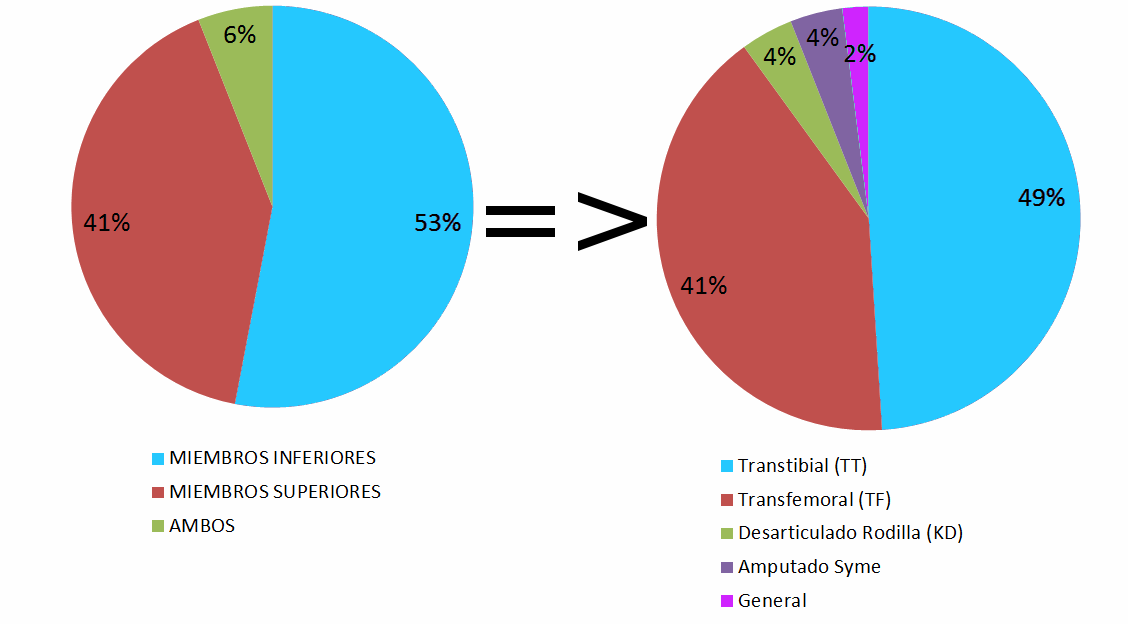
\includegraphics[scale=0.25]{Feathergraphics/Estadisticasestudios}
\par\end{centering}
\caption{Porcentaje de investigaciones en prótesis en los últimos 15 años \cite{Eshraghi2013}.}
\end{figure}
\end{frame}

\begin{frame}{Diabetes en el mundo}
\begin{columns}[t]


\column{40 mm}
%\begin{block}{}
{\footnotesize{}}

\begin{figure}
\begin{centering}
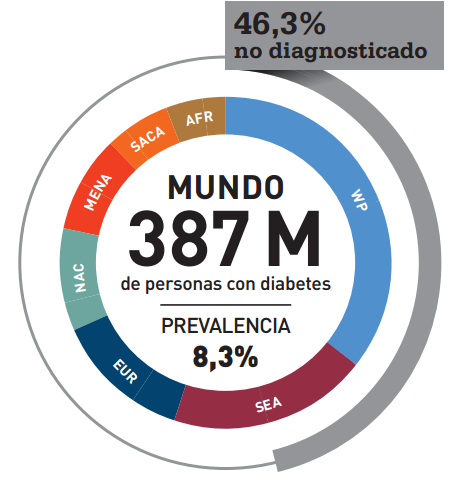
\includegraphics[scale=0.25]{Feathergraphics/proyecciondiabetes}
\par\end{centering}
\caption{Estadísticas de diabetes en el mundo \cite{ref1}.}
\end{figure}
%\end{block}

\column{75 mm}

%\begin{block}{}
\begin{figure}
\begin{centering}
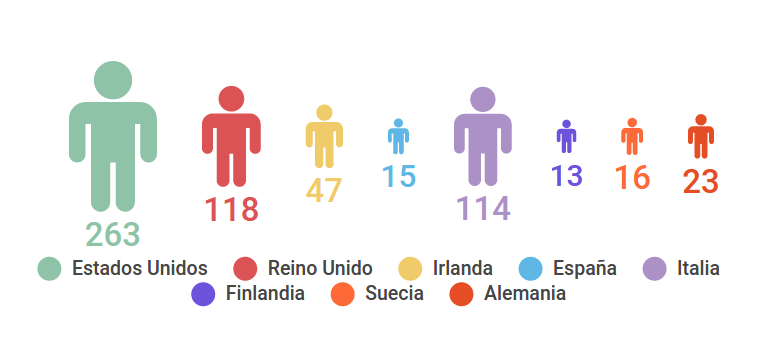
\includegraphics[scale=0.30]{Feathergraphics/ampperyear}
\par\end{centering}
\caption{Número de amputaciones por cada 100.000 habitantes. Adaptado de Kroger-Knut \cite{KrogerKnut2015}. }
\end{figure}

%\end{block}
\end{columns}

\end{frame}

\begin{frame}{Amputaciones en Colombia}{Factores}

\begin{columns}[t]


\column{70 mm}

\begin{figure}
\begin{centering}
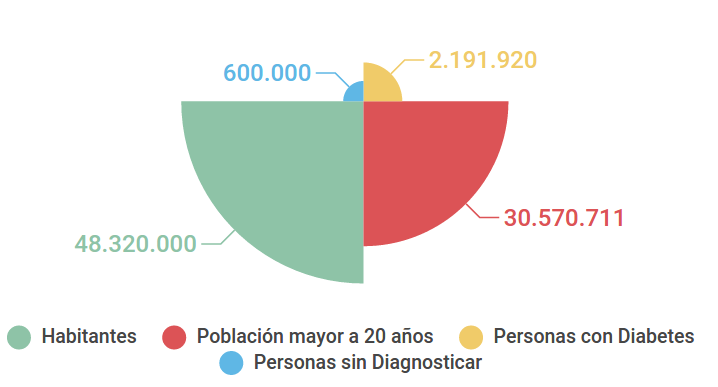
\includegraphics[scale=0.3]{Feathergraphics/DiabetesCol}
\par\end{centering}
\caption{{\scriptsize{}Diabetes en Colombia. Adaptado de Ramírez \cite{Ramirez2014}. }}

\end{figure}


\column{40 mm}
\begin{figure}
\begin{centering}
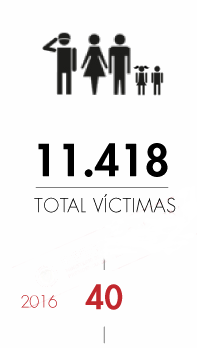
\includegraphics[scale=0.45]{Feathergraphics/TotalvictimasPAICMA}
\caption{{\scriptsize{}Situación víctimas MAP y MUSE a marzo de 2016\cite{PAICMA}}.}
\end{centering}
\end{figure}

\end{columns}

\end{frame}



\subsection{Avances en prótesis}
\begin{frame}{Estado actual prótesis comerciales}

\begin{figure}
\begin{centering}
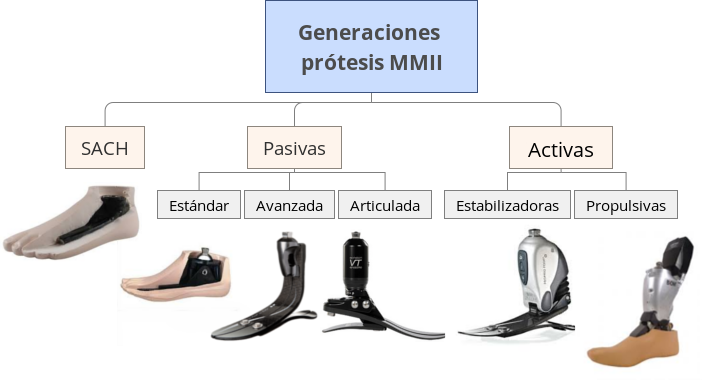
\includegraphics[scale=0.38]{Feathergraphics/Generacionesprotesis}
\par\end{centering}
\caption{{\footnotesize{}Categorización según Cherelle \emph{et al.} \cite{Cherelle2014a} de las
prótesis comerciales.} }

\end{figure}

\end{frame}


\section{Estado del conocimiento}

\begin{frame}{Fortalezas y debilidades prótesis pasivas}{Fortaleza prótesis ESR (\textit{Energy Storage and Return}) \cite{Zelik2014}, \\ Debilidades prótesis ESR \cite{Varol2010,Weber2014,Au2008,Morgenroth2011,Martinez-Villalpando2009,Esposito2015,DeAsha2014}}

\begin{columns}[t]

\column{55 mm}

\begin{figure}
\begin{centering}
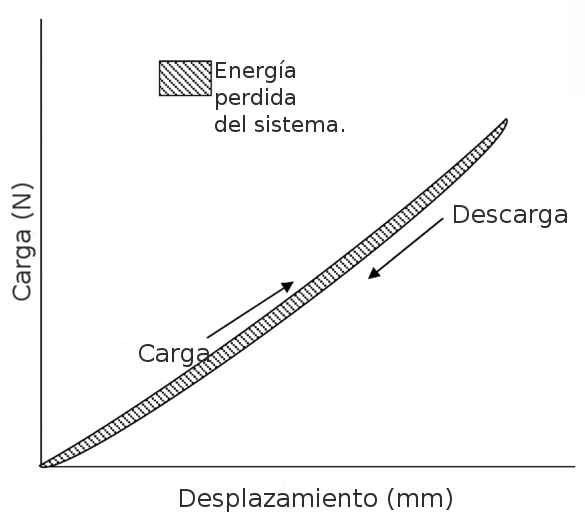
\includegraphics[scale=0.25]{Feathergraphics/hystheresis}
\par\end{centering}
\caption{\footnotesize{Histéresis CFRC a la compresión.\cite{Nolan2008}}}
\end{figure}

\column{50 mm}

%\begin{alertblock}{}

%\begin{itemize}
%\item {\footnotesize{Buena fuente de trabajo positivo al final de la fase
%de apoyo sin requerir baterías }\cite{Zelik2014}.}{\footnotesize \par}
%\item {\footnotesize{}Sólo reaccionan a la compresión en la etapa de dorsiflexión \cite{Varol2010}.}{\footnotesize \par}
%\item {\footnotesize{}Baja absorción al choque\cite{Au2008}.}{\footnotesize \par}
%\end{itemize}
%\end{alertblock}
\begin{figure}
\begin{centering}
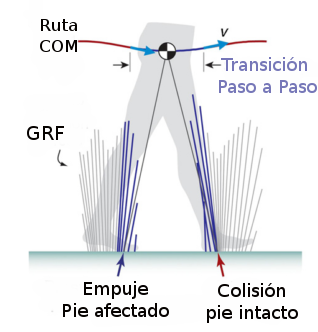
\includegraphics[scale=0.4]{Feathergraphics/colision}
\caption{\footnotesize{GRF del pie afectado y no afectado en amputado con prótesis pasivas \cite{Morgenroth2011}.}}
\end{centering}
\end{figure}

\end{columns}

\end{frame}

\begin{frame}{Alteraciones Biomecánicas prótesis ESR}{Patrones asimétricos}

\begin{alertblock}{}

\begin{itemize}
\item {\scriptsize{}Presentan patrones asimétricos en la marcha \cite{Au2009,Martinez-Villalpando2011,Hill2013a,Bateni2002}.}{\scriptsize \par}
\item {\scriptsize{}Susceptibilidad a la ósteoartritis de rodilla a largo
plazo \cite{Grabowski2013}.}{\scriptsize \par}
\item {\scriptsize{}Posible generador dolor dorso-lumbar \cite{Devan2014}.}{\scriptsize \par}
\end{itemize}
\begin{figure}
\begin{centering}
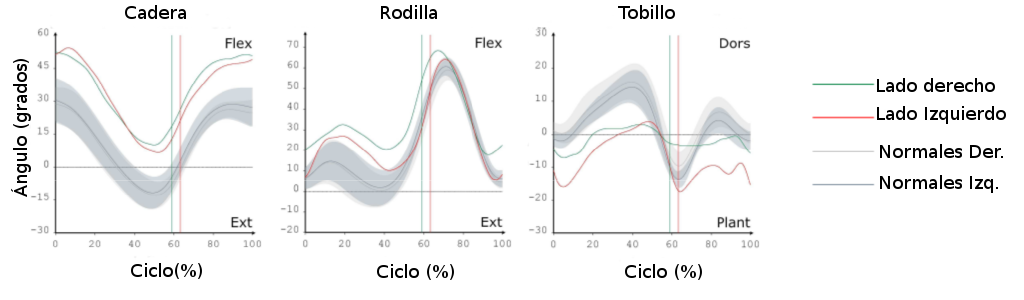
\includegraphics[scale=0.25]{Feathergraphics/Henry}
\par\end{centering}
\caption{Comportamiento cinemático caso clínico. Cortesía de UMB.}

\end{figure}

\end{alertblock}
\end{frame}

\begin{frame}{Consumo metabólico}{prótesis ESR vs Activas}

\begin{columns}[t]


\column{75 mm}
\begin{block}{}
{\footnotesize{}}

\begin{figure}
\begin{centering}
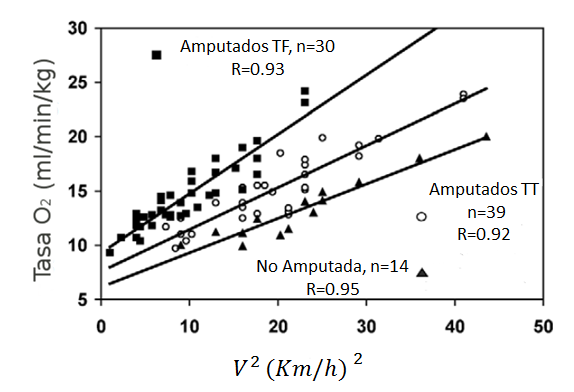
\includegraphics[scale=0.42]{Feathergraphics/consumo}
\par\end{centering}
\caption{{\footnotesize{}Consumo metabólico en amputados Trans-Femorales (TF) y Trans-Tibiales (TT) en comparación a la marcha no patológica. \cite{Schmalz2002}.}}\par
\end{figure}

\end{block}

\column{40 mm}
\begin{exampleblock}{}

\begin{itemize}
\item {\scriptsize{}ESR: Reducción velocidad de marcha (30\% a 40\%)\cite{Schmalz2002}.}{\scriptsize \par}
\end{itemize}
\vspace{12 mm}
\begin{itemize}
\item {\scriptsize{}Activas: Reducción de la demanda metabólica hasta 16\%
\cite{Herr2010,Esposito2015}.}{\scriptsize \par}
\end{itemize}
\vspace{12 mm}
\begin{itemize}
\item {\scriptsize{}Activas: Aumento en la velocidad preferida hasta en
un 10\% en comparación a las ESR\cite{Gates2013}.}{\scriptsize \par}
\end{itemize}
\end{exampleblock}
\end{columns}

\end{frame}

\begin{frame}{Cargas irregulares prótesis ESR vs. Activas}

\begin{columns}[t]


\column{60 mm}

\begin{figure}
\begin{centering}
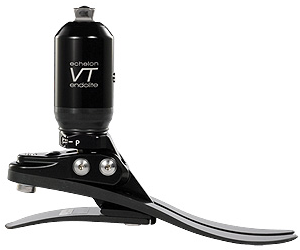
\includegraphics[scale=0.4]{Feathergraphics/echelon}
\par\end{centering}
\caption{Prótesis pasiva con actuador hidráulico.\cite{springking}}
\end{figure}


\column{60 mm}
\begin{exampleblock}{}

\begin{itemize}
\item {\footnotesize{}ESR: Crea resistencia a la rotación articular de tobillo
\cite{DeAsha2014}.}{\footnotesize \par}
\item {\footnotesize{}Activas: Reducciones en la presión pico en el contacto
de talón en comparación a las prótesis ESR \cite{Hill2013a}.}{\footnotesize \par}
\item {\footnotesize{}Activas: Decrecimientos en la fuerza resultante pico
y en los momentos aductores de rodilla del lado inafectado \cite{Grabowski2013}.}{\footnotesize \par}
\end{itemize}
\end{exampleblock}
\end{columns}

\end{frame}

\begin{frame}{Debilidades prótesis activas}

\begin{columns}[t]


\column{60 mm}
\begin{alertblock}{}

\begin{itemize}
\item {\scriptsize{}Causan altos niveles de ruido \cite{boston}.}{\scriptsize \par}
\item {\scriptsize{}No es escalable \cite{BIOMASME}.}{\scriptsize \par}
\item {\scriptsize{}No cumplen con el concepto de antropomorficidad\cite{BIOMASME}.}{\scriptsize \par}
\end{itemize}
\end{alertblock}
\begin{exampleblock}{}

\begin{itemize}
\item {\footnotesize{}El sistema reemplaza la pérdida muscular y tendinosa\cite{Varol2010}. }{\footnotesize \par}
\item {\footnotesize{}Reconoce diferentes terrenos y velocidades \cite{Lawson2011}. }{\footnotesize \par}
\item {\footnotesize{}Produce potencia positiva mecánica\cite{Martinez-Villalpando2009}.}{\footnotesize \par}
\end{itemize}
\end{exampleblock}

\column{60 mm}

\begin{figure}
\begin{centering}
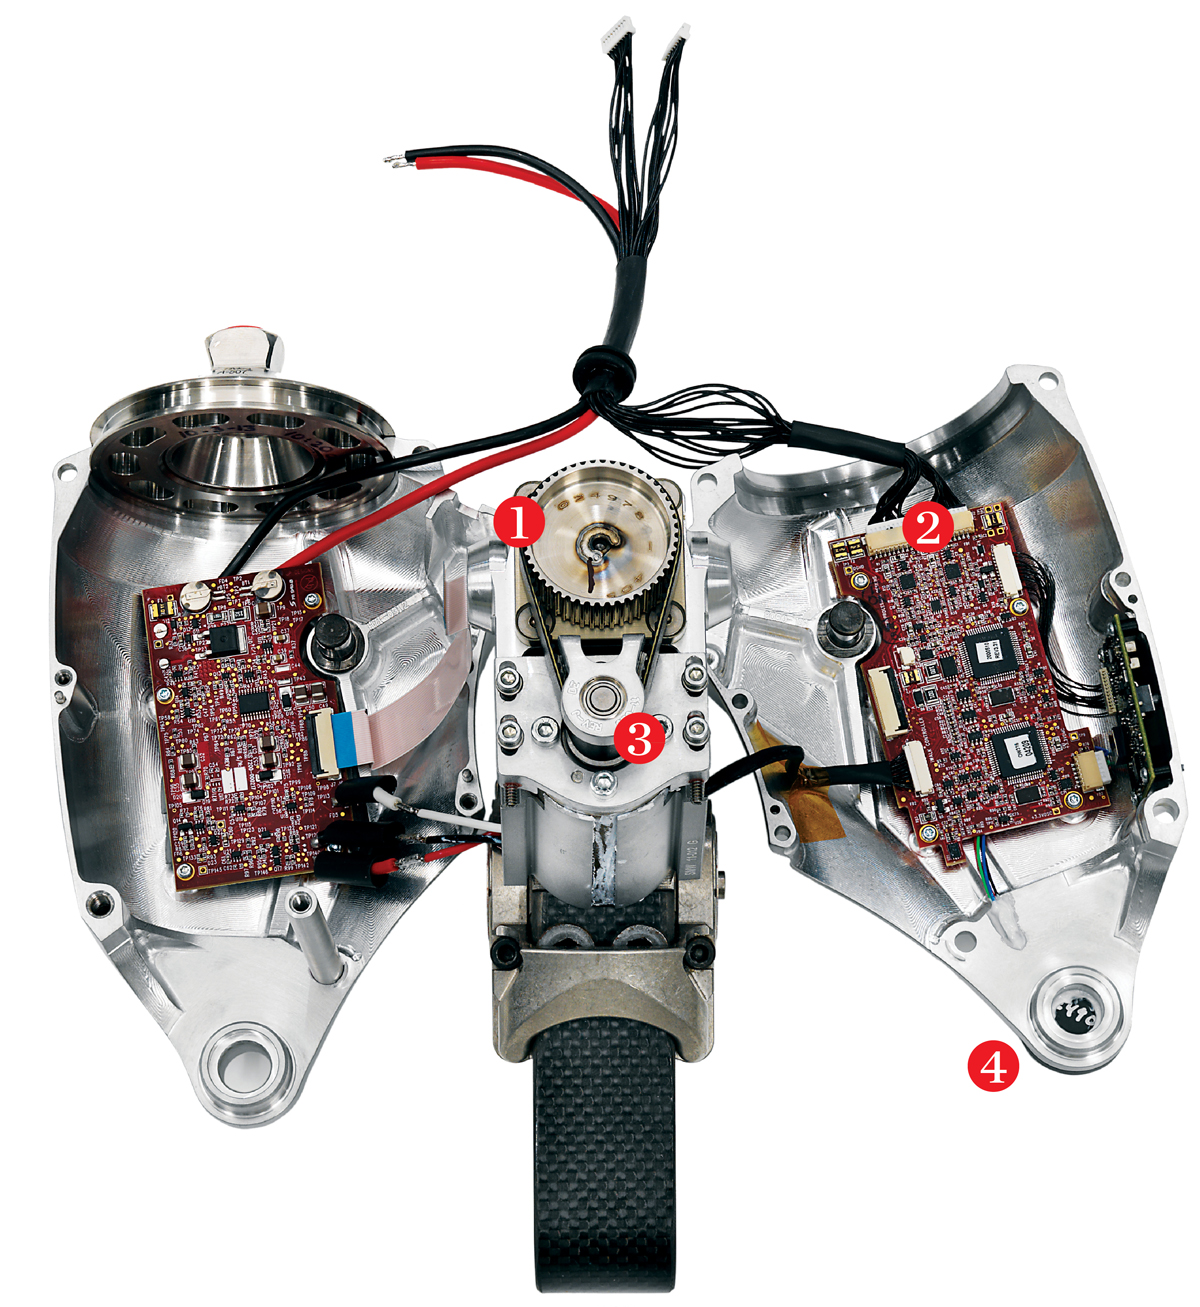
\includegraphics[scale=0.11]{Feathergraphics/Bionaked}
\par\end{centering}
{\scriptsize{}\caption{Configuración interna Biom \cite{boston}}
}{\scriptsize \par}

\end{figure}

\end{columns}

\end{frame}



\subsection{Problemática actual}
\begin{frame}{Demanda Energética}

\begin{figure}
\begin{centering}
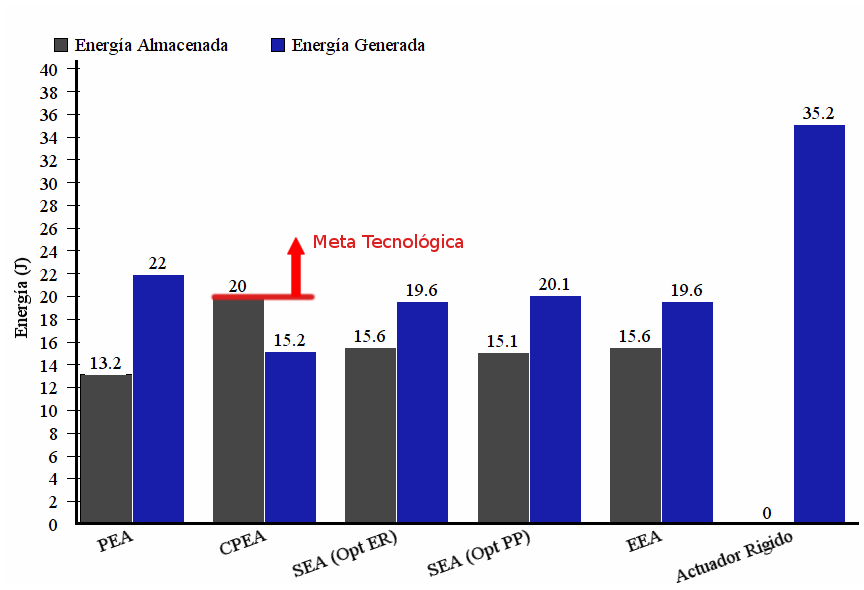
\includegraphics[scale=0.3]{Feathergraphics/20160113105227}
\caption{Energía almacenada vs Energía generada en actuadores protésicos \cite{Cherelle2014a}.}
\par\end{centering}
\end{figure}

\end{frame}

\begin{frame}{Torque, velocidad y potencia}

\begin{figure}
\begin{centering}
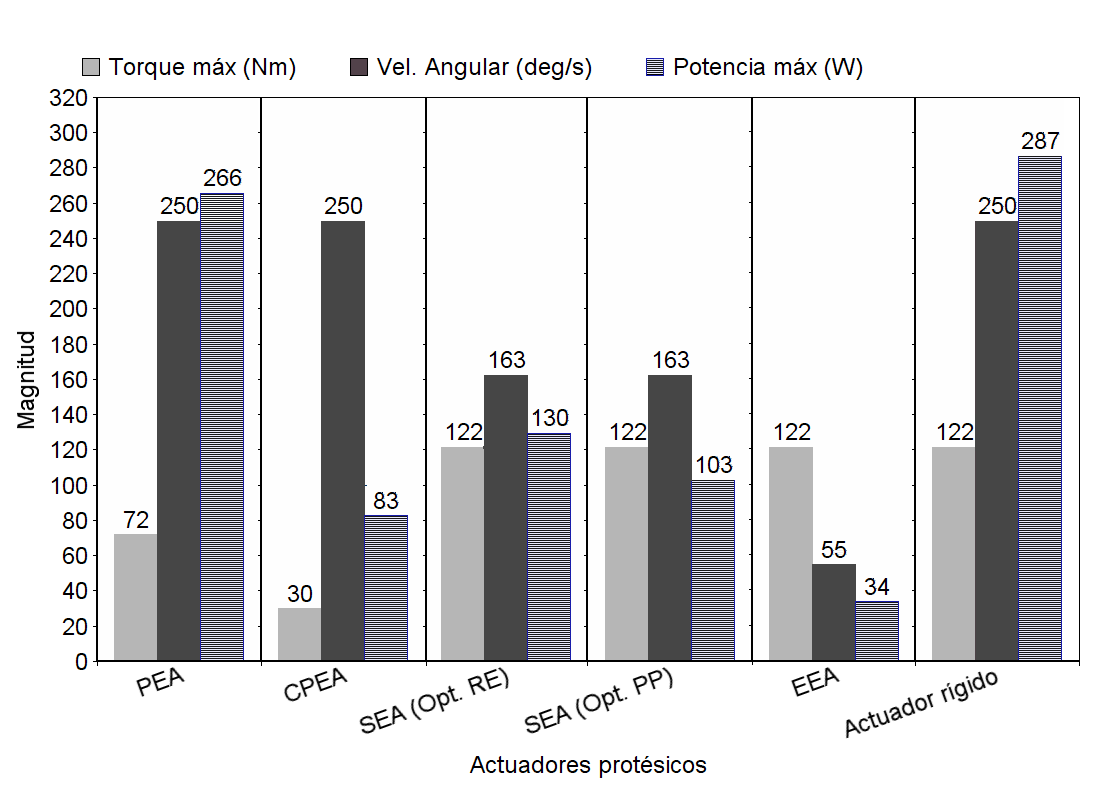
\includegraphics[scale=0.32]{Feathergraphics/20160414035751}
\par\end{centering}
\caption{Variables mecánicas actuadores protésicos \cite{Cherelle2014a}.}

\end{figure}

\end{frame}

\begin{frame}{Costos}

\begin{block}{Prótesis ESR son Económicas en relación a las activas}
\end{block}
\begin{figure}
\begin{centering}
\begin{tabular}{|c|c|c|c|}
\hline 
\multicolumn{2}{|c|}{Prótesis Pasivas} & \multicolumn{2}{c|}{Prótesis Activas}\tabularnewline
\hline 
\hline 
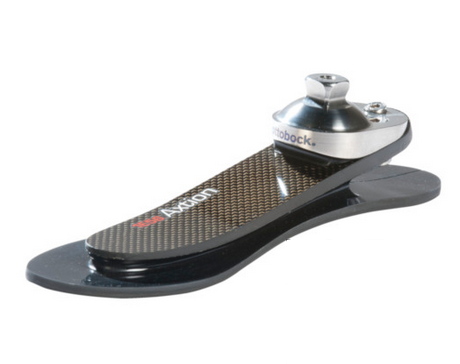
\includegraphics[scale=0.15]{Feathergraphics/axtion} & 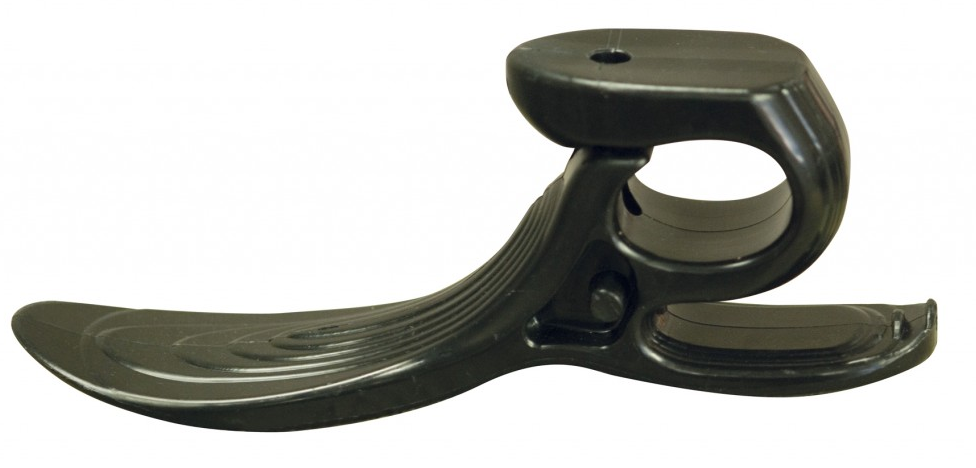
\includegraphics[scale=0.08]{Feathergraphics/niagara} & 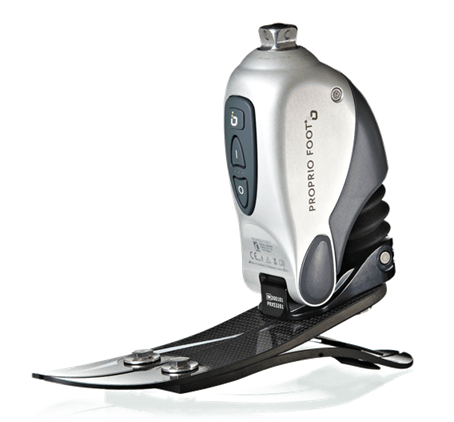
\includegraphics[scale=0.15]{Feathergraphics/proprio} & 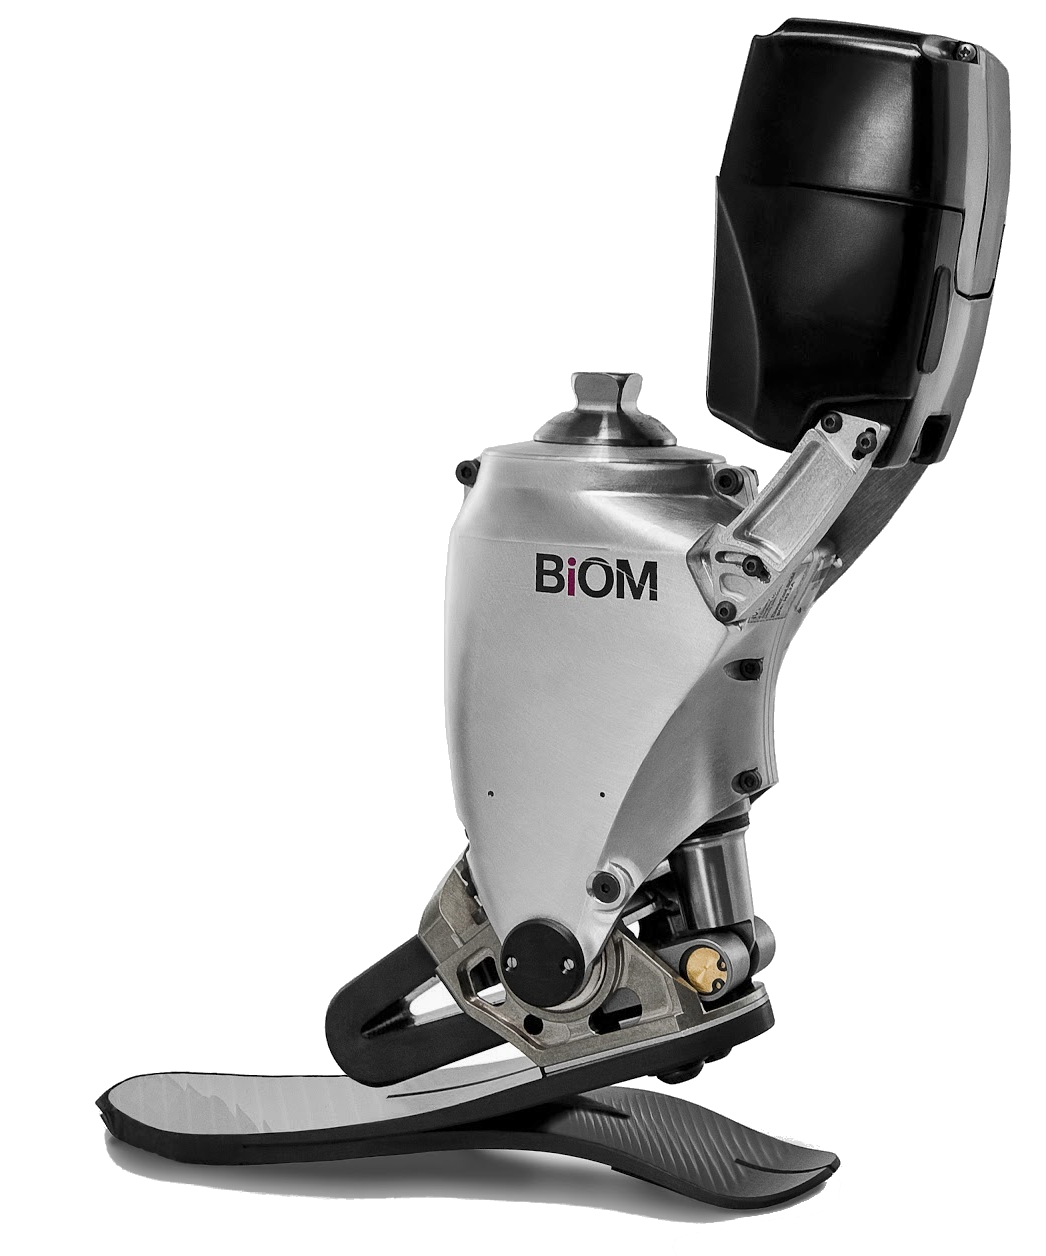
\includegraphics[scale=0.048]{Feathergraphics/BiOM}\tabularnewline
\hline 
{\footnotesize{}U\$1.034} & {\footnotesize{}U\$ 35\cite{Niagara}} & {\footnotesize{}U\$ 25.000 \cite{bloomberg}} & {\footnotesize{}U\$ 40.000 \cite{boston}}\tabularnewline
\hline 
\end{tabular}
\par\end{centering}
\caption{De Izq. a Der.: Axtion foot de OttoBock$\circledR$, Niagara foot,
Proprio Ossur$\circledR$ y Biom de Bionx$\circledR$. Imágenes obtenidas
de las páginas oficiales.}
\end{figure}

\end{frame}

\begin{frame}{Resumen comparativo}
\begin{table}
\begin{centering}
\caption{Resumen comparativo prótesis ESR vs Activas}
\begin{tabular}{|>{\centering}p{24mm}|>{\centering}p{45mm}|>{\centering}p{24mm}|}
\hline 
{\footnotesize{}Prótesis ESR} & {\footnotesize{}Aspecto} & {\footnotesize{}Prótesis Activas}\tabularnewline
\hline 
\hline 
{\footnotesize{}+25\%} & {\footnotesize{}Costo metabólico} & {\footnotesize{}+10\%}\tabularnewline
\hline 
{\footnotesize{}-30\%} & {\footnotesize{}Velocidad preferida} & {\footnotesize{}-10\%}\tabularnewline
\hline 
{\footnotesize{}$0.168 \pm 0.025 J/kg$} & {\footnotesize{}Transición de trabajo} & {\footnotesize{}$0.275 \pm 0.068 J/kg$}\tabularnewline
\hline 
{\footnotesize{}Mejores al SACH} & {\footnotesize{}Parámetros dinámicos} & {\footnotesize{}Mejores a las ESR}\tabularnewline
\hline 
{\footnotesize{}Cumple} & {\footnotesize{}Antropomorficidad} & {\footnotesize{}No cumple}\tabularnewline
\hline 
{\footnotesize{}No} & {\footnotesize{}Requerimientos energéticos externos} & {\footnotesize{}Si}\tabularnewline
\hline 
{\footnotesize{}Mayor} & {\footnotesize{}Presión contacto inicial} & {\footnotesize{}Menor}\tabularnewline
\hline 
{\footnotesize{}Mejor que SACH} & {\footnotesize{}Estabilidad} & {\footnotesize{}Mejor que ESR}\tabularnewline
\hline 
{\footnotesize{}Accesible} & {\footnotesize{}Precio} & {\footnotesize{}Elevado}\tabularnewline
\hline 
{\footnotesize{}No requiere} & {\footnotesize{}Mantenimiento} & {\footnotesize{}Requiere Sintonización}\tabularnewline
\hline 
\end{tabular}
\par\end{centering}


\end{table}

\end{frame}

\begin{frame}{Estrategias de Generación}

\begin{figure}
\begin{centering}
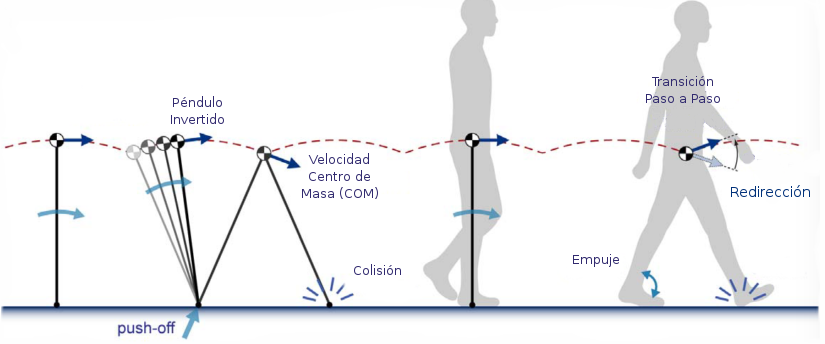
\includegraphics[scale=0.35]{Feathergraphics/transicion}
\par\end{centering}
\caption{Reciclaje de energía perdida en la marcha \cite{Collins2010}.}

\end{figure}
\end{frame}

\begin{frame}{Estrategias de Generación}

\begin{figure}
\begin{centering}
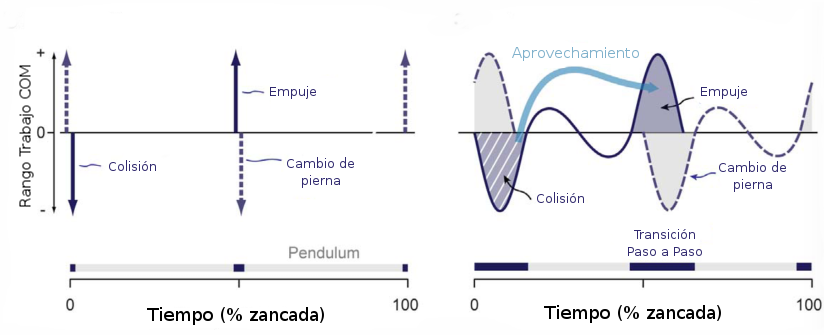
\includegraphics[scale=0.35]{Feathergraphics/transicion2}
\par\end{centering}
\caption{Transición de la energía perdida en la marcha \cite{Collins2010}.}
\end{figure}
\end{frame}

\begin{frame}{Fases de marcha unilateral}

\begin{center}
\begin{figure}
\begin{centering}
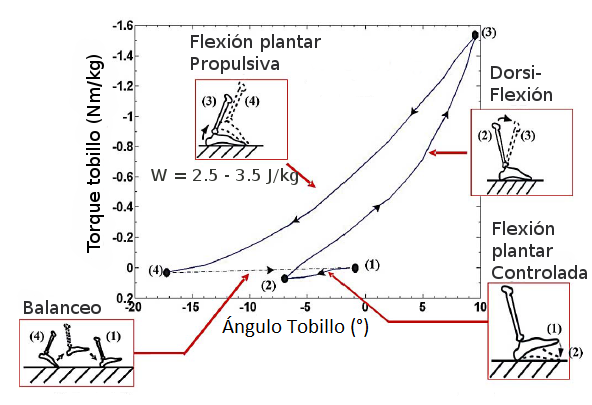
\includegraphics[scale=0.5]{Feathergraphics/cinneticatobillo}
\par\end{centering}
\caption{Comportamiento cinético y cinemático a replicar en el tobillo durante
la fase portante en la marcha normal \cite{Au2009}.}
\end{figure}
\par\end{center}

\end{frame}

\begin{frame}{Biomimetización}

\begin{columns}[t]


\column{65 mm}
\begin{block}{}
{\footnotesize{}}

\begin{figure}
\begin{centering}
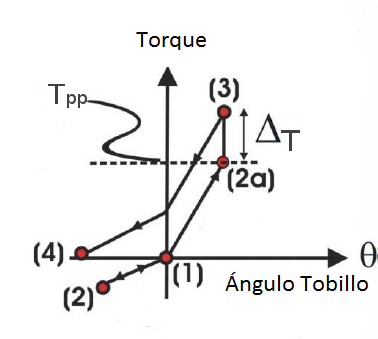
\includegraphics[scale=0.52]{Feathergraphics/cinneticatobillo3}
\par\end{centering}
\caption{{\scriptsize{}Generación del torque faltante en la marcha. \cite{Au2009} }}
\end{figure}

\end{block}

\column{50 mm}
\begin{exampleblock}{}

\begin{itemize}
\item {\footnotesize{}Prótesis ESR: No pueden replicar el trabajo positivo
generado en cada fase de la marcha humana \cite{Esposito2015}.}{\footnotesize \par}
\end{itemize}
\vspace{2 mm}
\begin{itemize}
\item {\footnotesize{}Prótesis Activas: requieren una mimetización más
detallada\cite{Hill2013a}.}{\footnotesize \par}
\end{itemize}
\vspace{2 mm}
\begin{itemize}
\item {\footnotesize{}Presenta una trayectoria más estable en comparación
a las pasivas\cite{Hill2013a}.}{\footnotesize \par}
\end{itemize}
\end{exampleblock}
\end{columns}

\end{frame}

%----------------------------------------------------------------
\section{Identificación del problema}

\subsection{Estrategias de generación de energía}

\begin{frame}{Relación problemática}

\begin{figure}
\begin{centering}
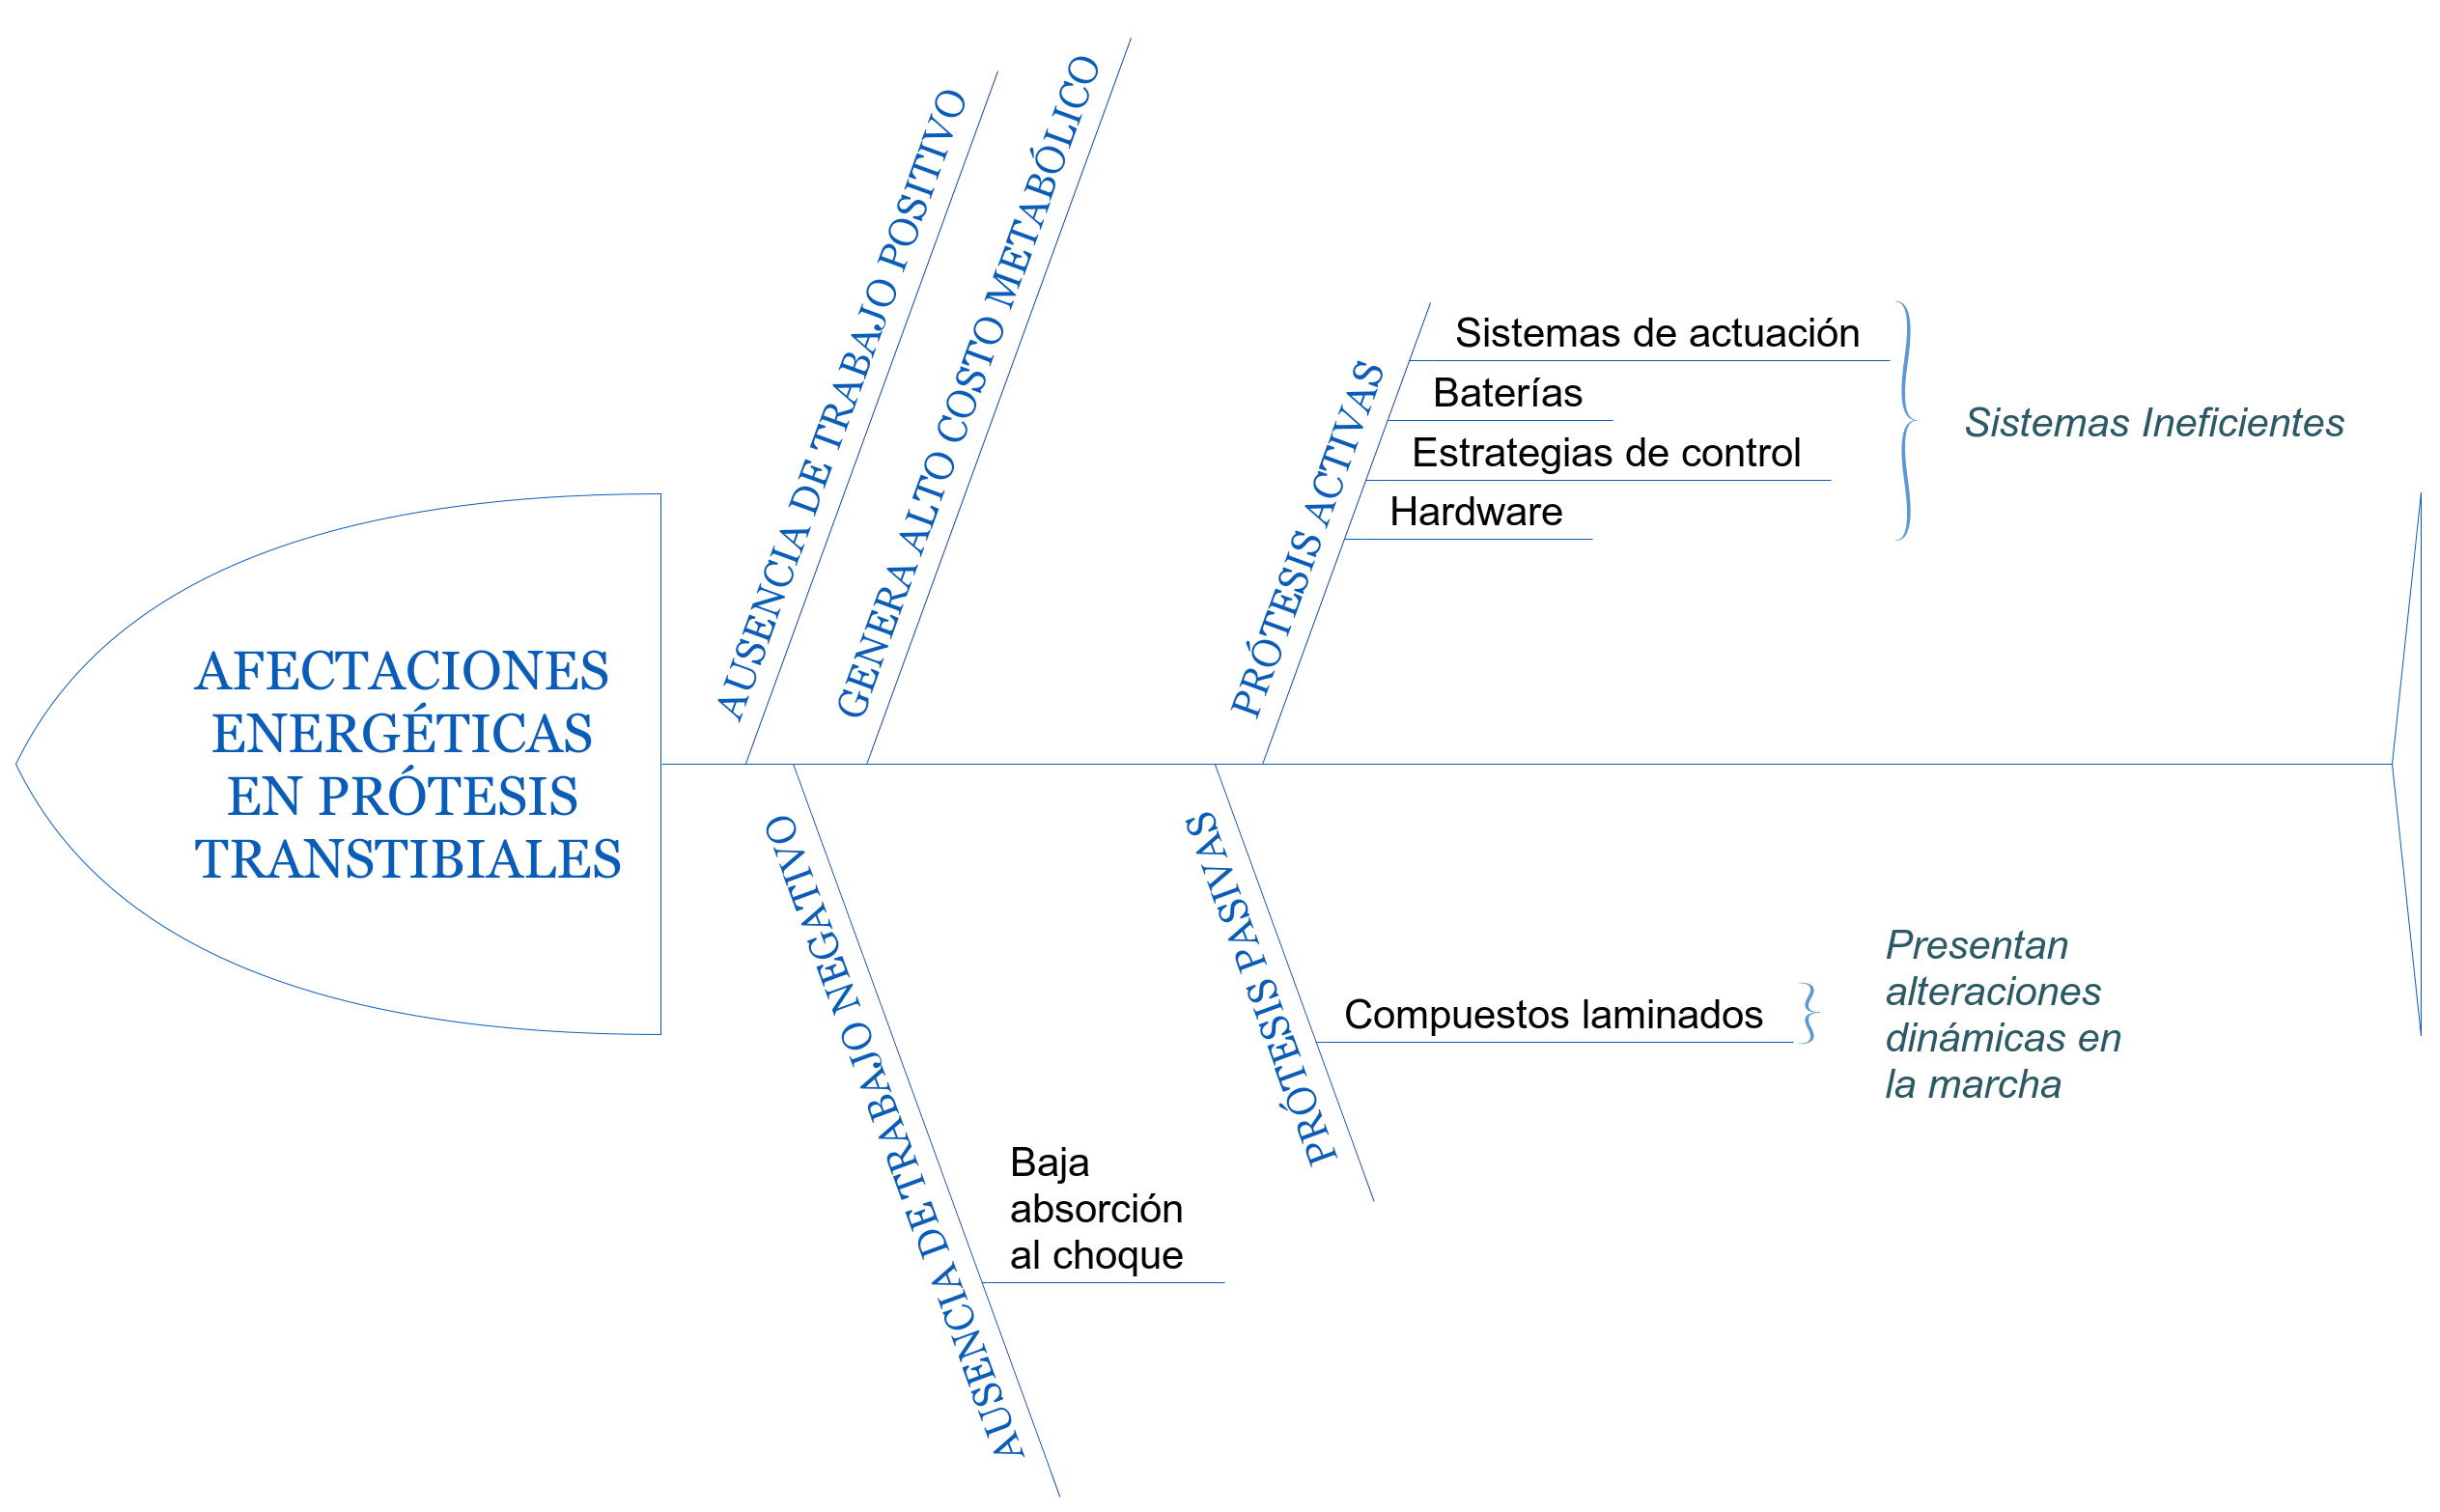
\includegraphics[scale=0.12]{Feathergraphics/AfectacionesEnergeticas.png}
\par\end{centering}
\caption{Mapa conceptual problemática}

\end{figure}

\end{frame}

\begin{frame}{Identificación del problema}

\begin{block}{Problemática actual}

Las prótesis pasivas actuales utilizadas en pacientes con amputación transtibial, provocan alteraciones en los parámetros dinámicos de la marcha para el amputado, debido a la ausencia de trabajo positivo del miembro faltante.

\end{block}
	\end{frame}


\subsection{Pregunta de investigación}
\begin{frame}{Identificación del problema}

\begin{block}{Pregunta de investigación}

¿Qué configuración de prótesis transtibial pasiva, generará el trabajo positivo necesario en la fase de apoyo final, a través del aprovechamiento de la energía perdida del Contacto Inicial de la marcha?

\end{block}
\begin{block}{Hipótesis}

Una prótesis transtibial, configurada para aprovechar la energía perdida del Contacto Inicial, permitirá generar el trabajo positivo necesario en la fase de apoyo final a través de un sistema dinámico pasivo.

\end{block}
\end{frame}

\section{Objetivos}

\subsection{Objetivo General}
\begin{frame}{Objetivos}

\begin{alertblock}{Objetivo General}

Proponer una configuración de prótesis transtibial, que genere a través de un
sistema dinámico pasivo, el trabajo positivo necesario en la dorsiflexión máxima, aprovechando la energía perdida en el contacto inicial de la marcha.
\end{alertblock}
\end{frame}


\subsection{Objetivos Específicos}
\begin{frame}{Objetivos}

\begin{exampleblock}{Objetivos específicos}

\begin{enumerate}
\item \small {Identificar los parámetros biomecánicos y el diagrama del ciclo de trabajo a usuarios de prótesis pasivas con amputación unilateral transtibial para determinar sus requerimientos energéticos.}
\item \small{Obtener el modelo preliminar de la prótesis transtibial que
aproveche la energía, durante el contacto inicial y el apoyo medio,
para entregarla en la fase de apoyo final de la marcha mediante un
sistema dinámico pasivo.}
\item \small{Determinar la configuración detallada del modelo preliminar de prótesis transtibial mediante la aplicación de sólidos celulares.} 
\item \small{Validar el modelo dinámico de la prótesis transtibial configurada, en comparación a un modelo protésico pasivo.}
\end{enumerate}
\end{exampleblock}
\end{frame}


\section{Metodología y actividades}
\subsection{Metodología general}
\begin{frame}{Metodología \emph{In Silico}}{Ciclo de validación}

\begin{figure}
\centering{}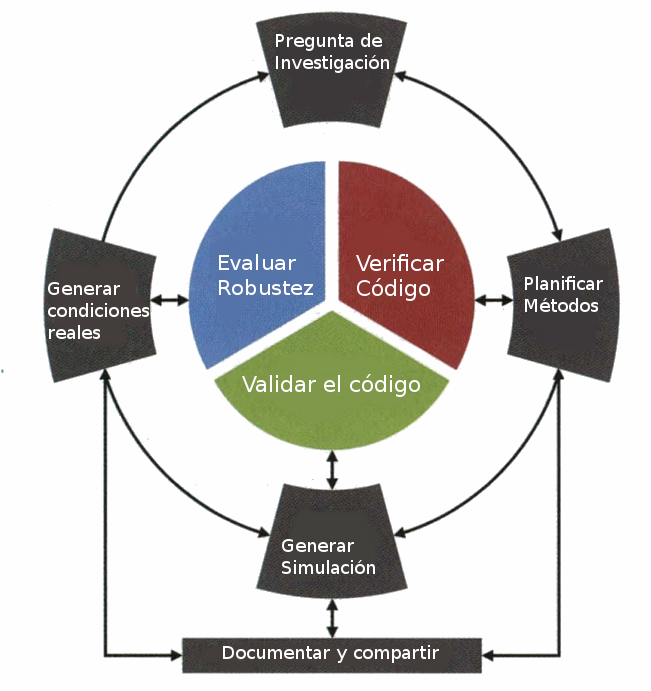
\includegraphics[scale=0.35]{Feathergraphics/verificationprocess}
\caption{{Proceso metodológico modelo \emph{In silico}. Tomado de  \cite{Hicks2014}.}}
\end{figure}

\end{frame}

\begin{frame}{Metodología \emph{In Silico}}{Marco computacional \emph{Open-source} tentativo.}
\begin{figure}[ht]
\begin{centering}
\begin{tikzpicture}[
    mindmap,
    every node/.style=concept,
    concept color=black!40,
    grow cyclic, text=white,
    level 1/.append style={level distance=2.2cm,sibling angle=90},
    level 2/.append style={level distance=1.8cm,sibling angle=45}, every node/.append style={scale=0.6}
    ]
  \node [root concept] {\Large{Python}} % root
    child [concept color=myblue] { node {Modelo biomecánico}
      child { node {Opensim} } 
      child { node {BTK} }
    }
    child [concept color=myblue] { node {Simulador FEM}
      child { node {Elmer} }
    }
    child [concept color=myblue] { node {Modelo multicuerpo}
      child { node {Simbody} }
      child { node {Pydy} }
    }
    child [concept color=myblue] { node {Visualizadores}
      child { node {VTK} }
      child { node {Paraview} }
    };
\end{tikzpicture}
%\caption{\label{Marco-computacional} Marco computacional \emph{Open-source} de la metodología tentativa a implementar en el proyecto.}
\end{centering}
\end{figure}

\end{frame}
\begin{frame}{Método Objetivo 1}{Recopilación variables de entrada}

\begin{block}{{\scriptsize{}Recopilar y/o adquirir los principales comportamientos
biomecánicos mencionados por Sagawa \emph{et al.} \cite{Sagawa2011} de la marcha estándar con amputación transtibial para realizar la modelación biomecánica a pacientes de prótesis ESR y a otros sujetos sin patologías.}}
\end{block}
\noindent \begin{center}
\begin{tabular}{|>{\raggedright}m{20mm}|>{\centering}p{25mm}|>{\centering}p{25mm}|}
\hline 
\multicolumn{3}{|c|}{{\tiny{} \textbf{Parámetros Biomecánicos}}}\tabularnewline
\hline 
{\tiny{} \textbf{Parámetros Espacio-temporales}} & {\tiny{} \textbf{Ángulos articulares}} & {\tiny{} \textbf{Potencia Articular}}\tabularnewline
\hline 
\hline 
\multirow{5}{20mm}{{\tiny{}Velocidad, cadencia, t. ciclo, t. fase apoyo, t. fase balanceo,
t. soporte simple...}} & {\tiny{}Ángulos de cadera, Rodilla y Tobillo} & {\tiny{}Cadera, Rodilla y Tobillo}\tabularnewline
\cline{2-3} 
 & {\tiny{}\textbf{Momentos articulares}} & {\tiny{}\textbf{Plataforma}}\tabularnewline
\cline{2-3} 
 & \multirow{3}{25mm}{{\tiny{}Cadera, Rodilla y Tobillo}} & \multirow{3}{25mm}{{\tiny{}Fuerza de Reacción anteroposterior, vertical y anteroposterior}}\tabularnewline
 &  & \tabularnewline
 &  & \tabularnewline
\hline 
\end{tabular}
\par\end{center}

\end{frame}

\begin{frame}{Actividades objetivo 1}{Adquisición variables dinámicas}

\begin{columns}[t]


\column{28 mm}
\begin{block}{}

\begin{itemize}
\item {\scriptsize{}Realizar solicitud comité de ética.}{\scriptsize \par}
\end{itemize}
\end{block}

\column{35 mm}
\begin{block}{}

\begin{itemize}
\item {\scriptsize{}Realizar protocolo adquisición de datos experimentales
en laboratorio de marcha.}{\scriptsize \par}
\vspace{5mm}
\item {\scriptsize{}Usuarios sin patologías y pacientes con amputación transtibial.}{\scriptsize \par}
\vspace{5mm}
\item {\scriptsize{}Toma de muestras con marcadores.}{\scriptsize \par}
\end{itemize}
\end{block}

\column{55 mm}
\begin{block}{}
\begin{figure}
\begin{center}
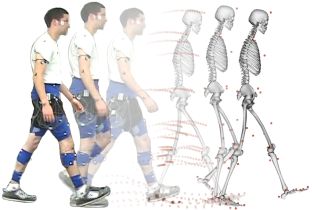
\includegraphics[scale=0.45]{Feathergraphics/labToModel}
\caption{\scriptsize{Proceso de traspaso variables temporales \cite{Seth2011}.}}
\end{center}
\end{figure}

\end{block}
\end{columns}

\end{frame}

\begin{frame}{Actividades Objetivo 1}{Dinámica inversa}

\begin{block}{\small{Obtener el modelo biomecánico computacional para calcular los parámetros no cuantificables directamente en laboratorio a través de la dinámica inversa.}}
\end{block}
\begin{columns}[t]
\column{60 mm}
%\begin{block}{}
\begin{figure}
\begin{centering}
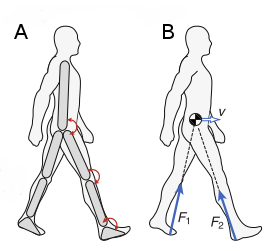
\includegraphics[scale=0.45]{Feathergraphics/RBvsLAB}
\par\end{centering}
\caption{\scriptsize {\scriptsize {Estimación de la colisión en la marcha \cite{Zelik2010}.}}}
\end{figure}
%\end{block}
\column{60 mm}
\begin{block}{\scriptsize {Ecuaciones de movimiento Newton-Euler}}
\begin{equation}
M(q)\ddot{q}+C(q,\dot{q})+G(q)=\tau
\end{equation}
\end{block}
\begin{block}{\scriptsize {Ecuaciones de movimiento de Lagrange}}
\begin{equation}
M^{i}\ddot{q}+K^{i}q^{i}+C_{q^{i}}^{T}\lambda=Q_{e}^{i}+Q_{v}^{i}
\end{equation}
\end{block}
\begin{block}{\scriptsize {Método de Kane}}
\begin{equation}
M(q,t)\dot{u}=f(q,\dot{q},u,t)
\end{equation}
\end{block}
\end{columns}
\end{frame}

\begin{frame}{Actividades Objetivo 1}{Obtención de la cuasi-rigidez}
\begin{columns}[t]
\column{60 mm}
\begin{figure}
\begin{center}
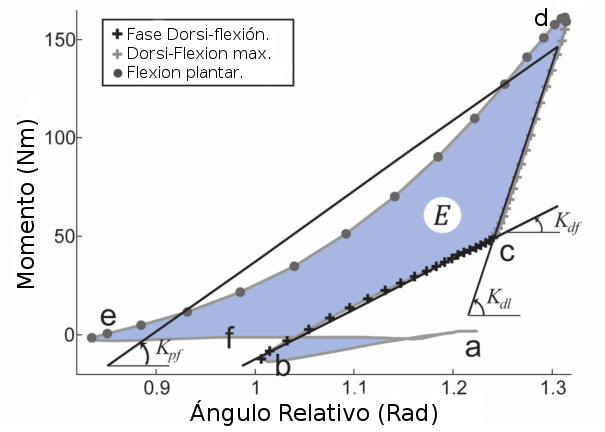
\includegraphics[scale=0.3]{Feathergraphics/quasirigidez}
\caption{Cuasi-rigidez de la articulación de tobillo \cite{Shamaei2013}.}
\end{center}
\end{figure}

\column{55 mm}
\vspace{10 mm}
\begin{block}{\scriptsize {Regresión lineal}}
\begin{equation}
\scriptsize {K_{pf}\thickapprox 11+\frac{34.6WH-3.81WHV-741}{\theta_{df}}}
\end{equation}
\begin{equation}
\tiny {K_{dl}\thickapprox \frac{-1596-(18.0V^{2}-88.8V+118.9)WHV+146.2W}{\theta_{dl}}}
\end{equation}
\begin{equation}
\scriptsize {K_{pf}\thickapprox 17-\frac{(3.68V-10.68)WHV^{3}-56.61W}{\theta_{pf}}}
\end{equation}
\end{block}


\end{columns}

\end{frame}
\begin{frame}{Método Objetivo 2}

\begin{columns}[t]


\column{60 mm}
\begin{block}
{\footnotesize{}Con herramientas para simulación dinámica multi-cuerpo deformable combinada con FEM, proponer la configuración del sistema global de la prótesis.}{\footnotesize \par}
\end{block}
%\begin{block}{\scriptsize {Matriz de gradientes}}
%\begin{equation}
%J=\frac{\partial{\xi}}{\partial{\bf{x}}}=\frac{\partial{\xi}}{\partial{\bf{\overline{x}}}}\frac{\partial\bf{\overline{x}}}{\partial{\bf{x}}}=\frac{\partial{\xi}}{\partial{\bf{\overline{x}}}}A^{T}
%\end{equation}
%\end{block}
\begin{block}{\scriptsize {Ecuaciones de movimiento de Lagrange}}
\begin{equation}
M^{i}\ddot{q}+K^{i}q^{i}+C_{q^{i}}^{T}\lambda=Q_{e}^{i}+Q_{v}^{i}
\end{equation}
\end{block}


\column{60 mm}

\begin{figure}
\begin{centering}
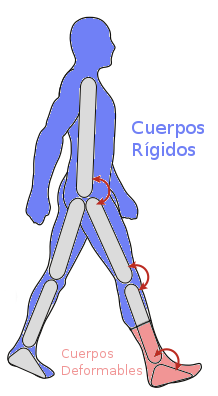
\includegraphics[scale=0.44]{Feathergraphics/deformable}
\caption{Adaptado de Zelik y Kuo \cite{Zelik2010}}
\par\end{centering}

\end{figure}

\end{columns}

\end{frame}

\begin{frame}{Actividades objetivo No. 2}


\begin{center}
\begin{figure}
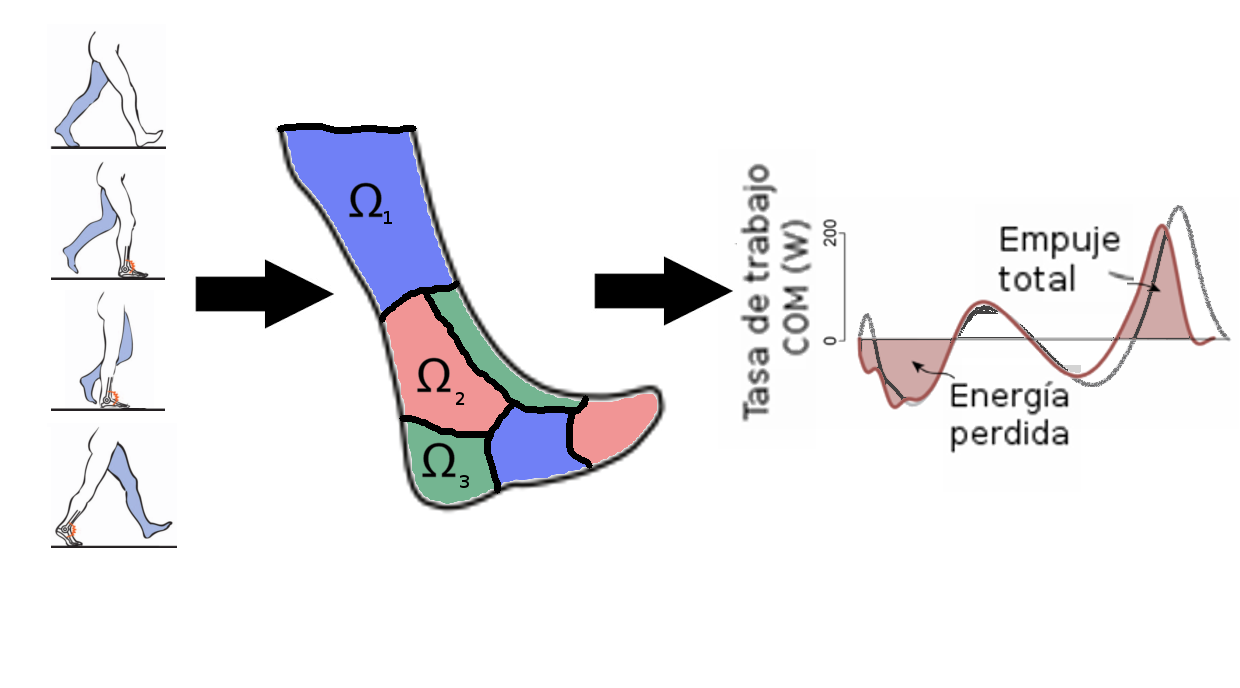
\includegraphics[scale=0.23]{Feathergraphics/Actividades2}
\caption{Proceso actividades objetivo 2. Adaptado de Shamaei \emph{et al.}\cite{Shamaei2013}, Collins y Kuo \cite{Collins2010} y Zelik \emph{et al.}\cite{Zelik2010}.}
\end{figure}
\end{center}
\end{frame}

\begin{frame}{Actividades objetivo No. 2}{Flujograma de proceso}
\begin{figure}
\begin{center}
\tikzset{decision/.style={diamond, draw, fill=blue!20, text badly centered,  node distance=2.5cm, inner sep=0pt,align=center}}
\tikzset{block/.style={rectangle, draw, fill=blue!20, text badly centered, rounded corners, minimum width= 4cm}}
\tikzset{line/.style={draw, very thick, color=black!50, -latex'}}
\tikzset{start/.style={shape=circle,draw,minimum size=1cm,draw=blue!80,fill=blue!20,text badly centered, align=center}}
\tikzset{stop/.style={shape=circle,draw,minimum size=1cm,draw=blue!80,fill=blue!20,text badly centered, align=center}}
\tikzset{decision answer/.style={near start,color=black}}
\begin{adjustbox}{max totalsize={.9\textwidth}{.7\textheight},center}
\begin{tikzpicture}[scale=2, auto, every node/.style={font=\Large, >=stealth,node distance=1cm,anchor=base,text width=7em}]

\node [start] (start){{\Large Inicio}}; 

\node [decision,text width=3cm,below=1cm of start] (buff) {{\Large Integrales de forma inerciales}}; 
\node [block,left=1cm of buff] (FEM){{\Large FEM }};
\node [block,right=1cm of buff] (analisis){{\Large Análisis estructural}};
\node [block,below=1cm of FEM] (CI){{\Large Lectura condiciones iniciales}};
\node [block,left=1cm of CI] (dinamica){{\Large Modelo Biomecánico}};
\node [block,below=1cm of CI] (matrices){{\Large Construcción de matrices}};
\node [block,below=1cm of matrices,text width=4cm] (integral){{\Large Integración de matrices en el tiempo}};
\node [stop,below=1cm of integral] (stop){Fin}; 
\node [decision,text width=3cm,left=1cm of stop] (overloop) {{\Large ¿Excede tiempo simulación?}};

\draw [line] (start) -- (buff);
\draw [line] (buff) -- (FEM);
\draw [line] (buff) -- (analisis);
\draw [line] (FEM) -- (CI);
\draw [line] (dinamica) -- (CI);
\draw [line] (CI) -- (matrices);
\draw [line] (matrices) -- (integral);
\draw [line] (integral) |- (overloop.north);
\draw [line] (overloop.east) -- node {no} (stop);
\draw [line] (overloop.west) |- node {yes} (matrices) ;


\end{tikzpicture}
\end{adjustbox}
\caption{Flujograma del algoritmo computacional. Adaptado de Shabana \cite{Shabana2013}.}
\end{center}
\end{figure}
\end{frame}

\begin{frame}{Metodología objetivo No. 3}

\begin{columns}[t]


\column{50 mm}
\begin{block}{{\footnotesize{}Ventajas de los sólidos celulares.}}

\begin{enumerate}
\begin{footnotesize}
\item Pueden soportar grandes deformaciones a bajos esfuerzos constantes \cite{Gibson1997}.
\item Posee buena relación masa-esfuerzo.
% \item Buena conductividad térmica \cite{Gibson1997}.
\end{footnotesize}
\end{enumerate}
\end{block}

\column{70 mm}

\begin{figure}
\begin{centering}
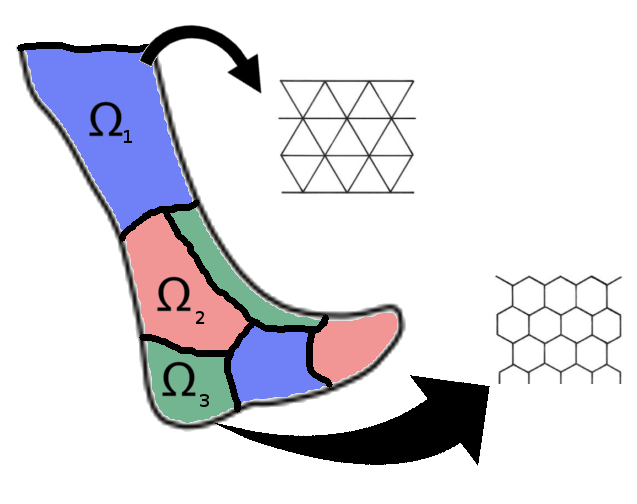
\includegraphics[scale=0.25]{Feathergraphics/honeycomb}
\par\end{centering}
\caption{{\scriptsize{Estrategia para llevar a cabo la fabricación. Adaptado de Zelik \cite{Zelik2010} y Gibson \cite{Gibson1997}.}}}
\end{figure}

\end{columns}

\end{frame}

\begin{frame}{Actividades objetivo No. 3}{Implementar materiales equivalentes que cumplan las propiedades elásticas}
\begin{columns}
\column {60 mm}

\begin{figure}
\begin{center}
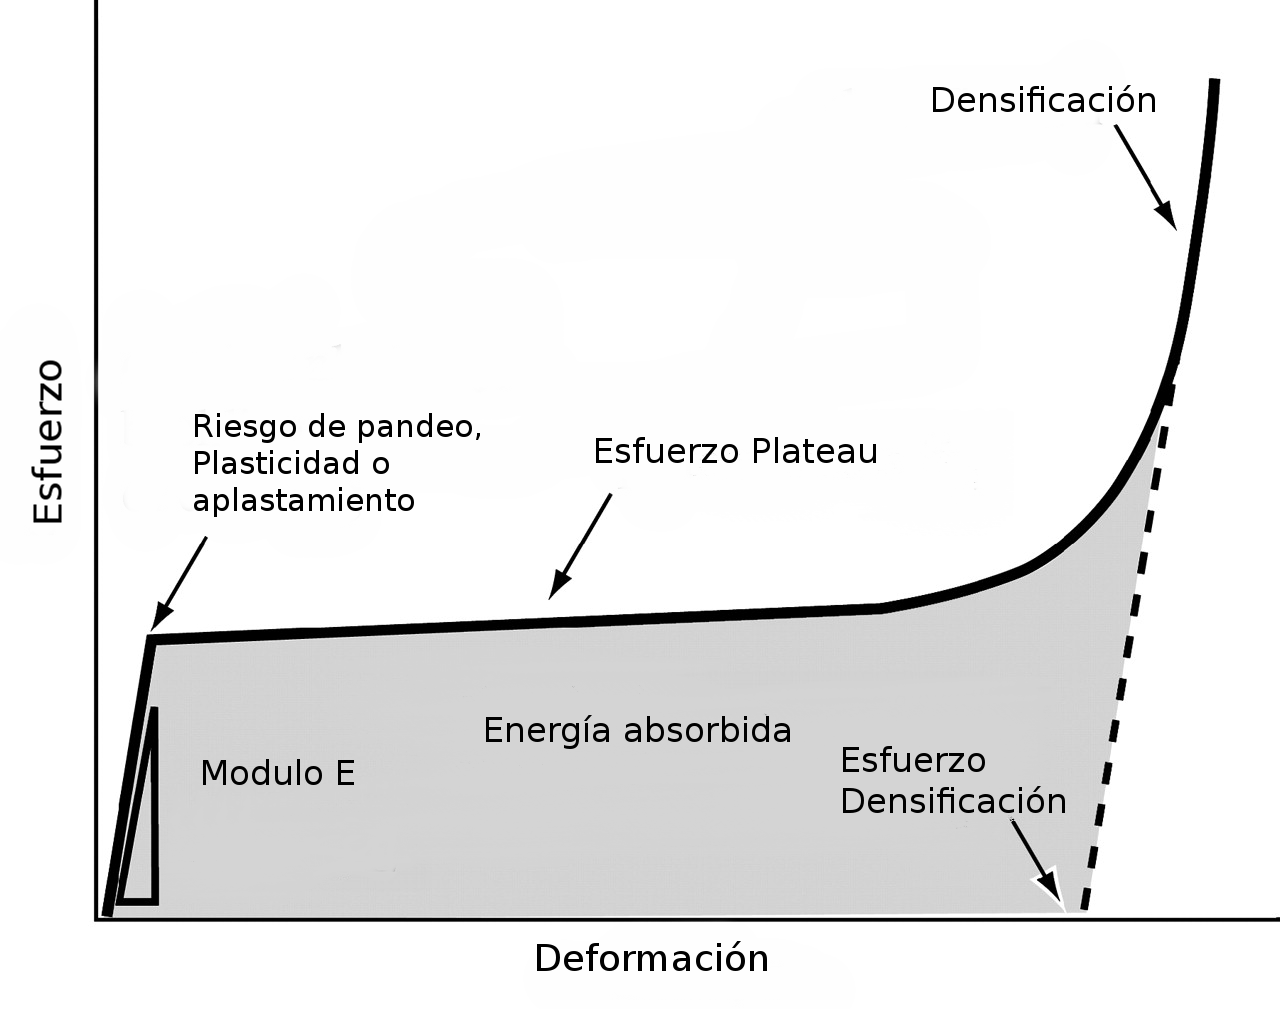
\includegraphics[scale=0.12]{Feathergraphics/compressioncellular}
\caption{{\footnotesize Comportamiento mecánico a la compresión en-plano para estructura celular. Adaptado de Ashby \cite{Ashby2006}.}}
\end{center}
\end{figure}

\column {65 mm}

\begin{figure}
\begin{centering}
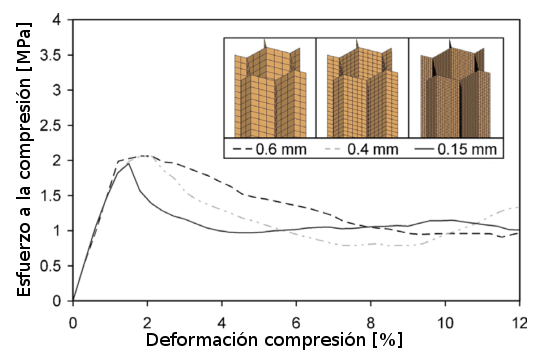
\includegraphics[scale=0.3]{Feathergraphics/stress-strainFEM}
\caption{{\footnotesize Comportamiento dinámico a la compresión de honeycombs. Adaptado de Heimbs \cite{Heimbs2009}.}}
\end{centering}
\end{figure}

\end{columns}
\end{frame}

\begin{frame}{Método objetivo No. 4}

\begin{block}{}{\begin{footnotesize}
Realizar la impresión 3D del modelo obtenido y validar el trabajo positivo generado del nuevo concepto mediante pruebas de marcha, comparándolos a su vez con un usuario sin
patologías.\end{footnotesize}}


\begin{figure}
\begin{centering}
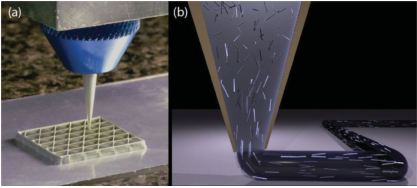
\includegraphics[scale=0.45]{Feathergraphics/3Dprinting}
\par\end{centering}
\caption{{\footnotesize Izquierda: Impresión 3D de una estructura \emph{Honeycomb} triangular con materiales compuestos. Derecha: Ilustración durante la deposición del compuesto. Tomado de Compton \cite{Compton2014}.}}

\end{figure}
\end{block}

\end{frame}

\begin{frame}{Actividades objetivo No. 4}

\begin{columns}[t]


\column{30 mm}
\begin{exampleblock}{}

\begin{itemize}[label={$\checkmark$}]
\item {\footnotesize{}Adaptación de los usuarios.}{\footnotesize \par}
\vspace{8 mm}
\item {\footnotesize{}Adquirir los parámetros biomecánicos.}
\vspace{8 mm}
\item {\footnotesize{Evaluar diferencias significativas.}}
\end{itemize}
\end{exampleblock}

\column{80 mm}

\begin{figure}
\begin{centering}
{\scriptsize{}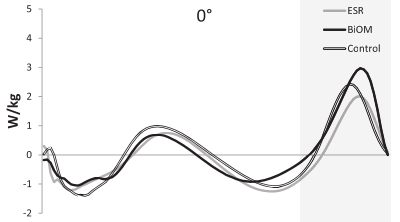
\includegraphics[scale=0.5]{Feathergraphics/biomvscontrolvsESR}}
\par\end{centering}{\scriptsize \par}
\caption{{\scriptsize{}Gráfica de potencia generada por kg en tres diferentes circunstancias. Tomado de Esposito \emph{et al.}\cite{Esposito2015}.}}
\end{figure}

\end{columns}

\end{frame}

\begin{frame}{Adquisición de parámetros mecánicos}{Implementación de técnicas ópticas sin contacto}
\begin{columns}
\column {70 mm}
\begin{figure}
\begin{centering}
\movie[label=show3,width=1.0\textwidth, poster
       ,autostart,showcontrols,loop, externalviewer] 
  {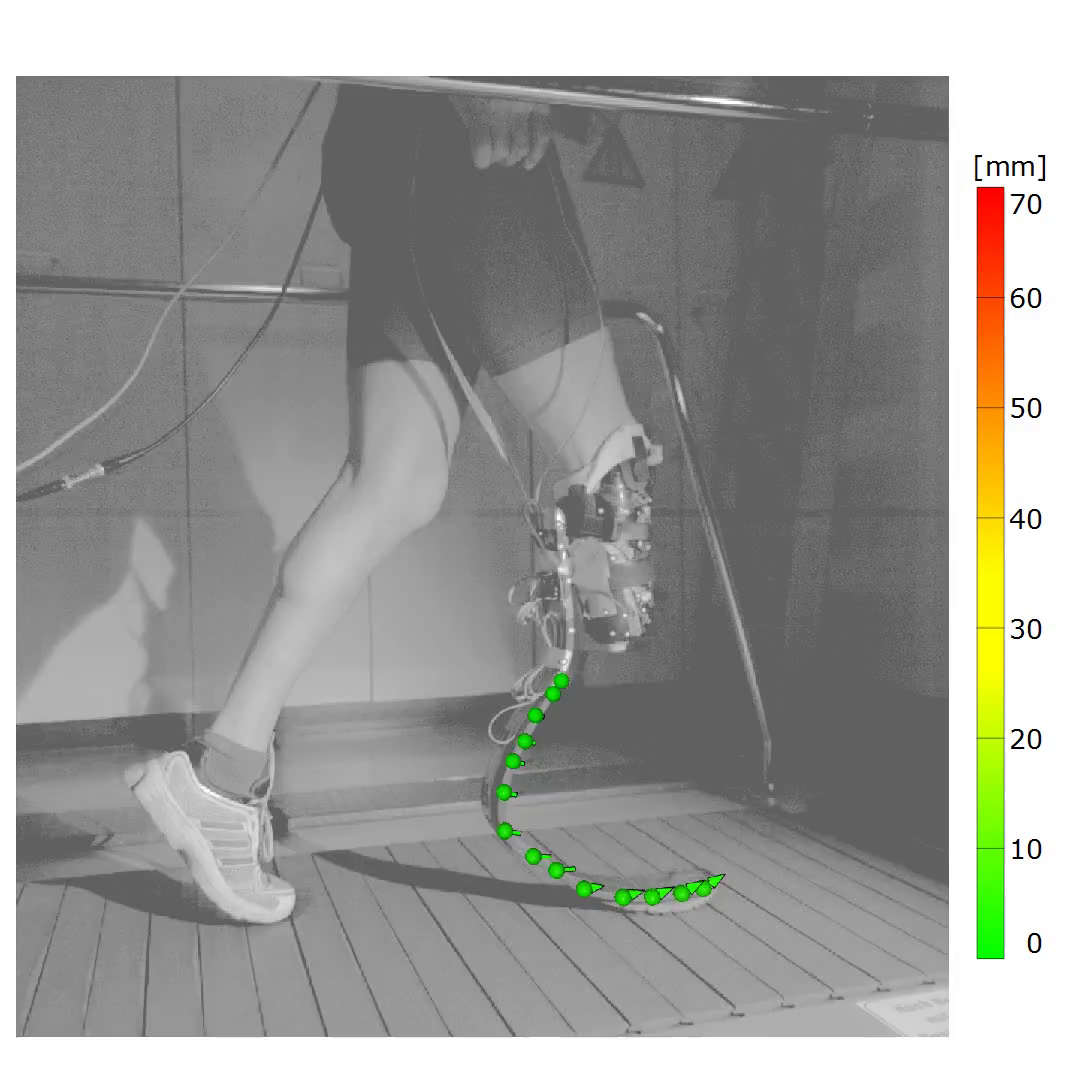
\includegraphics[width=0.75\textwidth]{Feathergraphics/displacement0.png}}{Feathergraphics/RunningProsthesis.avi}
\caption{{\footnotesize Prueba de carga cíclica en prótesis de alto impacto. Tomado de GOM \cite{GOM}.}}
\end{centering}
\end{figure}

\column {50 mm}

\begin{exampleblock}{}

\begin{itemize}[label={$\checkmark$}]
\item {\footnotesize{}Adquisición de deformaciones}{\footnotesize \par}
\vspace{8 mm}
\item {\footnotesize{}Adquisición de desplazamientos.}
\vspace{8 mm}
\item {\footnotesize{Cálculo del ciclo de vida.}}
\end{itemize}
\end{exampleblock}

\end{columns}

\end{frame}


\section{Cronograma y presupuesto}
\begin{frame}{Cronograma}

\begin{ganttchart}[
x unit=0.25cm,
y unit title=0.4cm,
y unit chart=0.45cm,
vgrid,
time slot format=isodate-yearmonth,
compress calendar,
title/.append style={draw=none, fill=myblue},
title label font=\footnotesize\sffamily\bfseries\color{white},
title label node/.append style={below=-1.6ex},
title left shift=.05,
title right shift=-.05,
title height=1,
bar/.append style={draw=none, fill=green!75},
bar height=.6,
bar label font=\normalsize\color{black!50},
group right shift=0,
group top shift=.6,
group height=.3,
group peaks height=.2,
bar incomplete/.append style={fill=brown}
]{2016-04}{2018-06}
\gantttitlecalendar{year} \\
\ganttbar[
progress=100,
bar progress label font=\small\color{white},
bar progress label node/.append style={right=4pt},
bar label font=\footnotesize\color{black!50},
name=pp
]{\scriptsize{Propuesta Doctoral}}{2016-04}{2016-06} \\
\ganttset{progress label text={}, link/.style={black, -to}}
\ganttgroup{\scriptsize{Objetivo 1}}{2016-06}{2016-10}\\ 
\ganttbar[progress=100, name=T1A]{\scriptsize{Adquisición parámetros dinámicos}}{2016-06}{2016-07} \\
\ganttbar[progress=80, name=T1A]{{\scriptsize Modelo Biomecánico rígido}}{2016-07}{2016-09} \\
\ganttgroup{{\scriptsize Objetivo 2}}{2016-10}{2017-05} \\
\ganttbar[progress=0, name=T2A]{{\scriptsize Modelo dinámico deformable}}{2016-10}{2017-05} \\
\ganttgroup{{\scriptsize Objetivo 3}}{2017-05}{2017-12} \\
\ganttbar[progress=0]{{\scriptsize Configuración sólido celular}}{2017-05}{2017-09}\\
\ganttbar[progress=0, name=T2A]{{\scriptsize Verificación FEM}}{2017-09}{2017-12} \\
\ganttgroup{{\scriptsize Objetivo 4}}{2017-10}{2018-04} \\
\ganttbar[progress=0]{{\scriptsize Impresión 3D}}{2017-10}{2018-01}\\
\ganttbar[progress=0, name=T2A]{{\scriptsize Validación experimental}}{2018-01}{2018-04} \\
\ganttgroup{{\scriptsize Escritura tesis y publicaciones}}{2016-10}{2018-06} \\
\ganttset{link/.style={black}}
%\ganttlink[link mid=.4]{pp}{T1A}
%\ganttlink[link mid=.159]{pp}{T2A}
\end{ganttchart}

\end{frame}

\begin{frame}{Presupuesto}{Presupuesto estimado global de la propuesta de investigación}

\begin{table}[H]
\noindent \centering{}{\scriptsize{}}%
\begin{tabular}{|>{\raggedright}p{33mm}|>{\centering}p{21mm}|>{\centering}p{25mm}|>{\raggedright}m{21mm}|}
\hline 
\multirow{2}{33mm}{{\scriptsize{}\textbf{Rubro}}} & \multicolumn{2}{c|}{{\scriptsize{}\textbf{Fuente}}} & \multirow{2}{21mm}{{\scriptsize{}\textbf{Subtotal}}}\tabularnewline
\cline{2-3} 
 & {\scriptsize{}\textbf{Interna}} & {\scriptsize{}\textbf{Externa}} & \tabularnewline
\hline 
\hline 
{\scriptsize{}\textbf{Personal}} & {\scriptsize{}\$26.319.000} & {\scriptsize{}\$144.000.000} & {\scriptsize{}\$ 170.319.000}\tabularnewline
\hline 
{\scriptsize{}\textbf{Equipo}} & {\scriptsize{}\$ 9.500.000} &  & {\scriptsize{}\$ 9.500.000}\tabularnewline
\hline 
{\scriptsize{}\textbf{Materiales}} &  & {\scriptsize{}\$10.000.000} & {\scriptsize{}\$ 10.000.000}\tabularnewline
\hline 
{\scriptsize{}\textbf{Salidas de campo}} &  & {\scriptsize{}\$ 5.000.000} & {\scriptsize{}\$ 5.000.000}\tabularnewline
\hline 
{\scriptsize{}\textbf{Capacitación}} &  & {\scriptsize{}\$ 41.600.000} & {\scriptsize{}\$ 41.600.000}\tabularnewline
\hline 
{\scriptsize{}\textbf{Publicaciones y patentes}} &  & {\scriptsize{}\$ 5.000.000}  & {\scriptsize{}\$ 5.000.000} \tabularnewline
\hline 
{\scriptsize{}\textbf{Servicios Técnicos}} &  & {\scriptsize{}\$ 10.000.000} & {\scriptsize{}\$ 10.000.000}\tabularnewline
\hline 
{\scriptsize{}\textbf{Viajes}} &  & {\scriptsize{}\$ 4.000.000} & {\scriptsize{}\$ 4.000.000} \tabularnewline
\hline 
{\scriptsize{}\textbf{Total}} & {\scriptsize{}\$ 35.819.000} & {\scriptsize{}\$ 219.600.000} & {\scriptsize{}\$ 255.419.000}\tabularnewline
\hline 
\end{tabular}
\end{table}

\end{frame}
\section{Implicaciones y Resultados esperados}

\begin{frame}{Impacto y Resultados esperados}
\begin{exampleblock}{}
\begin{itemize}[label={$\checkmark$}]
\item {\footnotesize{Nuevo concepto de almacenamiento de energía y devolución controlada.}}
%\vspace{8 mm}
\item {\footnotesize{Permitirá una antropomorficidad más detallada.}}
%\vspace{8 mm}
\item {\footnotesize{Permitirá realizar una metodología para la personalización de acuerdo a la antropometría y velocidad preferida del usuario.}}
%\vspace{8 mm}
\item {\footnotesize{Generará un mayor trabajo positivo en el despegue que una prótesis ESR.}}
\item {\footnotesize{Generará un modelo biomecánico específico para el estudio de caso.}}
\end{itemize}
\end{exampleblock}
\end{frame}
%\backupbegin
\begin{frame}[allowframebreaks]{Bibliografía}
%-------------------------------------------------------
\bibliographystyle{IEEEtran}
\tiny{\bibliography{Proposal.bib,patents.bib}}
\end{frame}
%\backupend

{\BiOM
\begin{frame}[plain,noframenumbering]
  \finalpage{Gracias!\\\emph{enprietop@unal.edu.co} \\ \emph{{\scriptsize In Memoriam: Elkin Gabriel Muskus Rincón}}}
\end{frame}}
% Appendix
\appendix
\newcounter{finalframe}
\setcounter{finalframe}{\value{framenumber}}
% Backup frames
\begin{frame}{Trabajos previos}

\begin{figure}
\begin{centering}
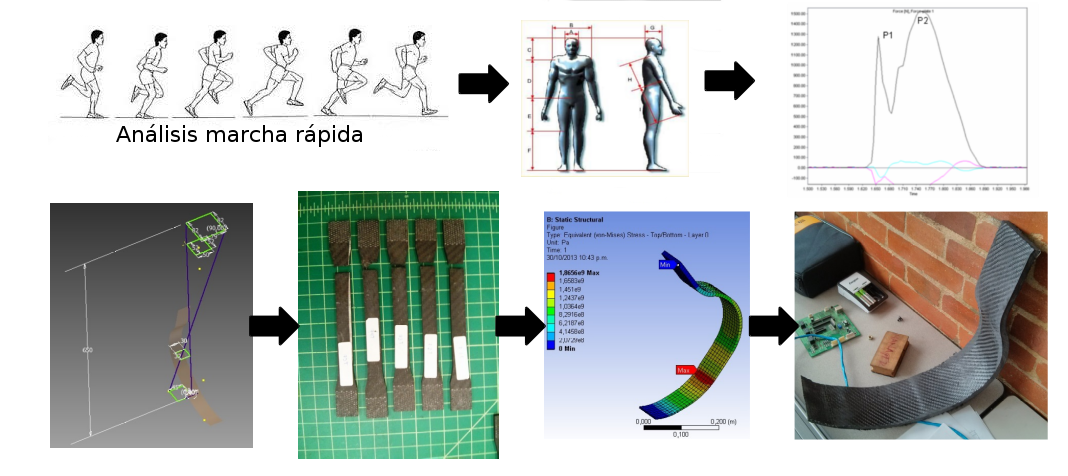
\includegraphics[scale=0.3]{Feathergraphics/tesismaestria}
\par\end{centering}
\caption{Desarrollo tesis de maestría. Imagen realizada por el autor}

\end{figure}

\end{frame}


\begin{frame}{Apéndice A}{Experiencia previa}

\begin{figure}
\begin{centering}
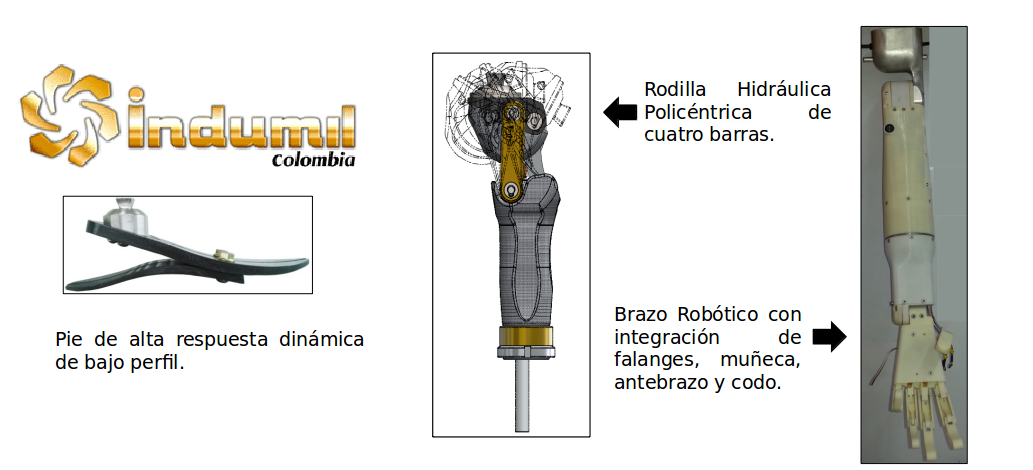
\includegraphics[scale=0.3]{Feathergraphics/experienciaIndumil}
\par\end{centering}
\caption{Experiencia en proyectos relacionados a la temática. Cortesía grupo
DAVINCI e INDUMIL.}

\end{figure}

\end{frame}

\begin{frame}{Apéndice B}{Estado actual actuadores protésicos}

\begin{tabular}{|>{\centering}p{20mm}|>{\centering}p{45mm}|>{\centering}p{35mm}|}
\hline 
\textbf{\small{}Tipo} & \textbf{\small{}Representación gráfica} & \textbf{\small{}Implementado en}\tabularnewline
\hline 
{\small{}SEA con transmisión continua variable} & {\small{}\vspace{1 mm}}{\small \par}

{\small{}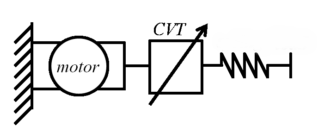
\includegraphics[scale=0.35]{Feathergraphics/CVSEA}} & {\small{}No implementado a la fecha.}\tabularnewline
\hline 
{\small{}SEA con elasticidad en paralelo} & {\small{}\vspace{1 mm}}{\small \par}

{\small{}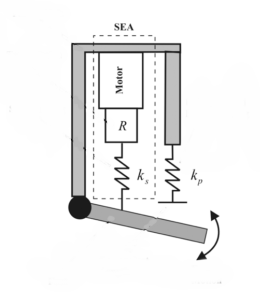
\includegraphics[scale=0.35]{Feathergraphics/BiOMmodel}} & {\small{}Pie BiOM de iWalk $\circledR.$\cite{herr2011controlling,herr2014powered,han2012controlling,han2014controlling}}\tabularnewline
\hline 
\end{tabular}
\end{frame}

\begin{frame}{Apéndice B}{Estado actual actuadores protésicos}

\begin{tabular}{|>{\centering}p{20mm}|>{\centering}p{40mm}|>{\centering}p{30mm}|}
\hline 
\textbf{\footnotesize{}Tipo } & \textbf{\footnotesize{}Representación gráfica} & \textbf{\footnotesize{}Implementado en}\tabularnewline
\hline 
\hline 
{\footnotesize{}Actuador elástico con amortiguador en serie (SEDA)} & {\footnotesize{}\vspace{1 mm}}{\footnotesize \par}

{\footnotesize{}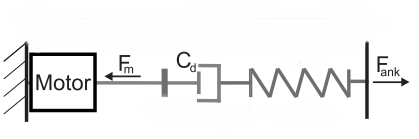
\includegraphics[scale=0.3]{Feathergraphics/SEDA}} & {\footnotesize{}No implementado \cite{Eslamy2013}.}\tabularnewline
\hline 
{\footnotesize{}Actuador elástico con amortiguador en paralelo (PEDA)} & {\footnotesize{}\vspace{1 mm}}{\footnotesize \par}

{\footnotesize{}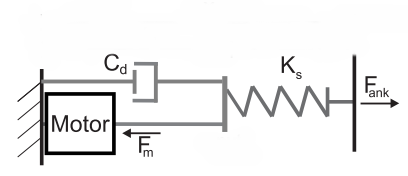
\includegraphics[scale=0.3]{Feathergraphics/PEDA}} & {\footnotesize{}No implementado \cite{Eslamy2013}.}\tabularnewline
\hline 
{\footnotesize{}Actuador de Rigidez Variable} & {\footnotesize{}\vspace{1 mm}}{\footnotesize \par}

{\footnotesize{}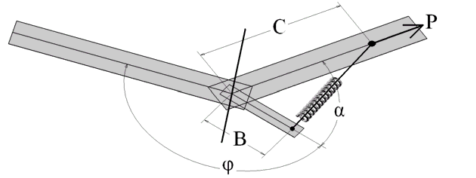
\includegraphics[scale=0.25]{Feathergraphics/maccepa2}} & {\footnotesize{}Proyecto CYBERLEG. \cite{Cherelle2014}}\tabularnewline
\hline 
\end{tabular}
\end{frame}

\begin{frame}{Apéndice B}{Estado actual actuadores protésicos}

\begin{tabular}{|>{\centering}p{20mm}|>{\centering}p{30mm}|>{\centering}p{45mm}|}
\hline 
\textbf{\scriptsize{}Tipo} & \textbf{\scriptsize{}Representación gráfica} & \textbf{\scriptsize{}Implementado en}\tabularnewline
\hline 
\hline 
{\scriptsize{}Actuador rígido} & {\scriptsize{}\vspace{1 mm}}{\scriptsize \par}

{\scriptsize{}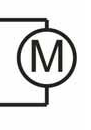
\includegraphics[scale=0.4]{Feathergraphics/DD}} & {\scriptsize{}Proprio Ossur $\circledR$}\tabularnewline
\hline 
{\scriptsize{}Actuador Elástico en Serie (SEA)} & {\scriptsize{}\vspace{1 mm}}{\scriptsize \par}

{\scriptsize{}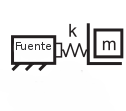
\includegraphics[scale=0.6]{Feathergraphics/SEAmodel}} & {\scriptsize{}-SPARKy (Spring Ankle with Regenerative Kinetics) \cite{Holgate2008,Bellman2008}.}{\scriptsize \par}

{\scriptsize{}-Prototipo transfemoral de la U. Vanderbilt.\cite{Sup2008,Sup2009}}\tabularnewline
\hline 
{\scriptsize{}SEA con Embrague (CSEA)} & {\scriptsize{}\vspace{1 mm}}{\scriptsize \par}

{\scriptsize{}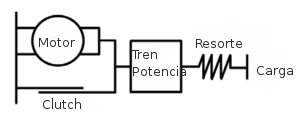
\includegraphics[scale=0.35]{Feathergraphics/CSEA}} & {\scriptsize{}Prototipo de rodilla de iWalk$\circledR$.}\tabularnewline
\hline 
\end{tabular}
\end{frame}
\begin{frame}{Apéndice C}{Biomecánica de la marcha}
\begin{columns}
\column{75 mm}
\begin{figure}
\begin{centering}
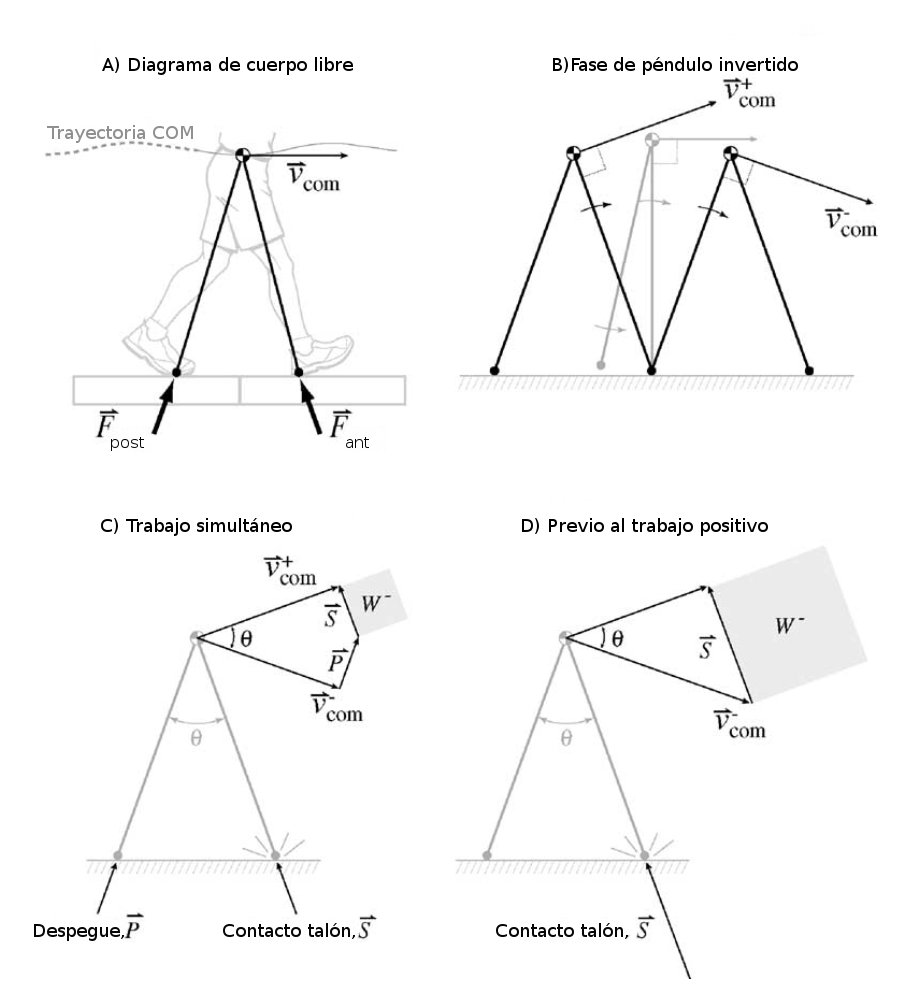
\includegraphics[scale=0.18]{Feathergraphics/workLL}
\par\end{centering}
\caption{Modelo biomecánico de Donelan y Kuo \cite{Donelan2002}.}
\end{figure}
\column{45 mm}
\begin{block}{{\footnotesize Potencia mecánica}}
\begin{footnotesize}
\begin{equation}
P_{ant}=F_{ant}\cdot\overrightarrow{v_{com}}
\end{equation}
\begin{equation}
P_{pos}=F_{pos}\cdot\overrightarrow{v_{com}}
\end{equation}
\end{footnotesize}
\end{block}
\begin{block}{{\footnotesize Trabajo mecánico externo}}
\begin{footnotesize}
\begin{equation}
W_{pos\&ant}=\intop_{pos\&ant}P_{pos\&ant}dt
\end{equation}
\begin{equation}
W_{tot}^{+}=W_{ant}^{+}+W_{pos}^{+}
\end{equation}
\begin{equation}
W_{tot}^{-}=W_{ant}^{-}+W_{pos}^{-}
\end{equation}
\end{footnotesize}
\end{block}
\end{columns}
\end{frame}
\setcounter{framenumber}{\value{finalframe}}

\end{document}
